\documentclass[11pt]{article}
\usepackage{geometry}
\geometry{verbose,letterpaper}
\usepackage{movie15}
\usepackage{hyperref}
\usepackage{graphicx}
\usepackage{epsfig}
\usepackage{longtable}
\usepackage{booktabs}
\usepackage{rotating}
\usepackage{times}
\usepackage{amssymb}
\usepackage{amsmath}
%\usepackage{subfigure}
\usepackage[colon]{natbib}
\usepackage{epsfig}
\usepackage{graphicx}
\usepackage{fullpage}
\usepackage{setspace}
\usepackage{authblk}
\usepackage{color}
\usepackage{array}
\usepackage{booktabs}
\usepackage{dcolumn}
\usepackage{multirow}
\usepackage{indentfirst}
\usepackage[toc,page]{appendix}
%\usepackage{titlesec}
\renewcommand{\baselinestretch}{1.31}
\newcommand\ddfrac[2]{\frac{\displaystyle #1}{\displaystyle #2}}
\usepackage{caption}
\renewcommand\theContinuedFloat{\alph{ContinuedFloat}}
\usepackage[labelsep=endash]{caption}
\DeclareCaptionLabelFormat{UC}{\textsc{#1} #2}
\captionsetup{labelformat=UC} % for all labels
\def\E{\mathcal{E}}

\usepackage{subcaption}
\renewcommand\thesubfigure{(\alph{subfigure})}
\captionsetup[sub]{
  labelformat=simple
}


\newcommand{\red}[1]{\textcolor{red}{#1}}

\newcommand{\argmax}{\operatornamewithlimits{argmax}} 
%\doublespacing

\begin{document}

\title{Speculative Bubbles and Market Segmentation}

\author[a]{Efthymios G Pavlidis} 
\author[a]{Kostas Vasilopoulos}

\affil[a]{\small{Department of Economics, Lancaster University Management School,
Lancaster, UK}}

\date{}
\maketitle

\begin{abstract}
We propose a novel approach for testing for rational speculative bubbles in segmented capital markets. The basic idea is that, under capital controls, heterogeneity of speculative expectations across international equity markets causes financial assets with identical cash flow promises to trade at different prices. Because these deviations from the law of one price inherit the properties of the speculative bubble process, they display periods of explosive dynamics and have predictive power for future movements in equity prices in sample. These two hypotheses can be examined empirically using sequential unit root tests and predictive regressions. An attractive feature of this approach for bubble detection is that it does not require the specification of a model for market fundamentals, thus mitigating the well-known joint hypothesis problem. The focus of the paper is on mainland Chinese companies that cross list shares in Hong Kong. China is an ideal setting for our analysis because of the significant restrictions on capital movements imposed by the authorities and the turbulent behavior of its stock market over the last decades.
\begin{flushleft}
\textbf{Keywords:} speculative bubbles; law of one price; AH premium; recursive unit root tests; predictive regressions    
\newline
 \textbf{JEL Classification:} C22, C32, G15
\end{flushleft}
\end{abstract}


\section{Introduction}

\begin{center}
\textit{China's stock market: A crazy casino} (The Economist, May 26$^{\text{th}}$ 2015)
\vspace{-.1cm}
\end{center}
\paragraph{} Since the re-opening of the Shanghai stock exchange (SSE) and the foundation of the Shenzhen stock exchange (SZSE) in the early 1990s, the Chinese stock market has experienced a remarkable growth. Starting from just a handful of listed companies in 1990 and a tiny market capitalization, it expanded to over three thousand firms in 2017 and a market capitalization of seven trillion dollars, ranking second worldwide behind the United States \citep{carpenterW2017}. While the Chinese stock market has grown rapidly over the last decades, movements in Chinese share prices have been anything but tranquil, with spectacular price rallies followed by severe market crashes occurring in the 1990s, 2000s, and 2010s. Such extreme financial events appear difficult to explain using observed market fundamentals and have led to a consensus that speculative forces are in action in the Chinese stock market. Notably, in his 2001 speech, the preeminent Chinese economist Wu Jinglian compared China's stock market to a \textit{casino}, that is manipulated by speculators and lacks a strong link to fundamentals. The \textit{casino} term has since been adopted by the popular press to describe the overall behaviour of Chinese share prices. Given China's leading role in global economic growth and investment, the presence of speculative dynamics, bubbles, in the country's capital allocation system constitutes a topic of increasing significance. 

In general, testing for speculative bubbles in financial markets is confounded by the fact that the fundamental value of financial securities is unobserved. Early studies have attempted to address this issue by utilizing observed variables, such as dividends, to estimate intrinsic values. A major drawback of such direct approaches is that they depend crucially on the strong and, in most cases, unrealistic assumption that the true data generating process for fundamentals is known. As argued by several researchers, model misspecification or omitted variables can lead to false inference in favour of bubbles, rendering direct approaches invalid \citep{HamiltonW1985,floodG1994,Gurkaynak2008}. To circumvent this problem, more recent studies have employed indirect approaches that exploit information about market fundamentals incorporated in derivative prices or survey data \citep{pavlidisPPf2017,pavlidisPP2018}. These studies show that periodically collapsing bubbles create a wedge between actual realizations of future spot prices and market expectations which, under general conditions, depends solely on the bubble process. As an implication, rather than using estimates of intrinsic asset values to assess the presence of speculative bubbles, researchers can examine the dynamics of the difference between actual future spot prices and market expectations. Unfortunately, indirect approaches based on future prices or survey data cannot be applied in the case of China because derivative markets are at an early stage of development and survey data on market expectations that cover periods long enough to allow a proper econometric analysis do not exist.\footnote{Equity warrants were briefly introduced in China in 2005--8 \citep{liuZZ2014}. By examining the behavior of the warrants market during this period, \citet{XiongY2011} provide strong evidence in favour of speculative dynamics. Specifically, they show that the price of many put warrants with long maturities exceeded both the upper bound given by the strike price and the more conservative fundamental value implied by the Black and Scholes model.}  


In this paper, we propose an alternative approach for testing for rational speculative bubbles that makes use of the unique trading features of Chinese cross-listed securities. There is a large number of companies incorporated in mainland China that simultaneously issue A shares on SSE or SZSE, and H shares on the Stock Exchange of Hong Kong (SEHK). For a given issuer, these two types of shares have identical voting rights and exchange-rate-adjusted dividend payments (i.e., they have the same fundamentals) but differ in terms of their accessibility by different groups of investors. Prior to the introduction of the Stock Connect scheme in 2015, Chinese mainland investors could easily access A but not H shares, while international and Hong Kong investors could readily access H but not A shares because of strict government regulations. The segmentation of A- and H-share markets implied that price valuations of the same security could differ across geographical locations without giving rise to arbitrage opportunities \citep{chenK1995,frootD1999,LamontT2003}. The main idea of the present paper is that, in this setting with limits to arbitrage, differences in speculative trading in Chinese mainland and Hong Kong can lead to distinct bubbles processes in A- and H-share markets. As a consequence, share prices of cross-listed companies can diverge despite having the same underlying fundamentals.

To demonstrate the theoretical implications of different speculative dynamics in A- and H-share markets, we adopt a standard asset-pricing model with rational, risk-neutral investors and consider  a periodically collapsing bubble process in the market for A but not for H shares. We show that, in this framework, the A-H price differential displays two characteristic properties when the bubble erupts. First, the price differential grows (in expectation) at an exponential rate, thus displaying explosive dynamics and, second, it has predictive content for future changes in A-share prices. These two properties can be examined empirically to test for speculative bubbles by exploiting recent advances in recursive unit root tests and in predictive regression tests with persistent regressors.

%. We examine the former property by   using the popular recursive unit root testing procedure of \citet{PhillipsSY2015a,PhillipsSY2015b}. For the latter property, we employ a rolling, predictive-regression framework in which we draw statistical inference using the IVX method of \citet{PhillipsM2009} and \citet{KostakisMS2015}. %This method is appealing because it allows for regressors displaying various degrees of persistence, from stationary to mildly explosive (references!!). 

For our empirical application, we use data on the Hang Seng AH Premium Index and on a panel of 27 cross-listed companies spanning the period from January 2006 to December 2016. By employing the popular Generalized Supremum Augmented Dickey Fuller (GSADF) of \citet{PhillipsSY2015a,PhillipsSY2015b} and its panel version, we show that A-H price differentials display episodes of explosive dynamics. These episodes are relative short and coincide with periods commonly considered to be characterized by speculative bubbles. Namely, the Chinese stock market \textit{frenzy} of 2007 and the Chinese Stock market \textit{crash} of 2014-2015. A similar conclusion is reached by looking at the predictive regression results, which indicate periods of in-sample predictability, again, during 2007 and 2014-15. Overall, in line with the \textit{casino} hypothesis, our findings support the presence of speculative dynamics in the Chinese stock market.

The presence of distinct bubble processes in mainland China and Hong Kong provides a possible explanation for one of the most intriguing puzzles in finance: the large and highly persistent share price deviations of Chinese cross-listed companies \citep{fernaldR2002,carpenterW2017}. In addition to speculation, a number of other factors have been put forth in the literature to explain foreign share discounts, such as different attitudes toward risk, information asymmetries, changes in exchange rate expectations, liquidity and transaction costs \citep{wangJ2004,chanMY2008,chungHL2013}. As a final exercise, we use a dynamic panel probit methodology to investigate whether such factors can explain the identified episodes of exuberance in A-H price differentials. 

The rest of the paper is structured as follows. Section \ref{sec:instit} provides an overview of the institutional background of Chinese stock markets. Section \ref{sec:theory} outlines the theoretical framework and describes the proposed bubble detection methods. The following section deals with the empirical application of these methods to A-H cross-listed shares. The same section  provides a robustness exercise based on American Depository Receipts, and also presents the results of the dynamic panel probit analysis. The final section concludes.


\section{Institutional Background}\label{sec:instit}

China's modern stock market opened only in the early 1990s with the re-establishment of SSE on November 26, 1990 and the foundation of the SZHE on December 1, 1991. %Over the last four decades, these two exchanges have experienced spectacular growth. 
Upon their opening, SSE listed eight companies and had a market capitalization of 1.2 billion renminbi (RMB), and SZHE listed six companies with a total share capital of 273 million RMB. By 2016, the number of listings in SSE and SZHE increased to 3,134 firms and their combined market capitalization reached 51 trillion RMB, which corresponded to 68 percent of the country's gross domestic product. 

There are two types of tradable shares issued by Chinese firms listed on SSE and SZHE, the so-called A and B shares. The market for A shares is by far the largest, accounting for the lion's share of trading volume and market capitalization. A shares are quoted in domestic currency (RMB) and, until recently, were primarily traded by mainland Chinese citizens due to strict capital controls imposed by the Chinese authorities.\footnote{During our sample period, China implemented a number of schemes aiming to gradually open its capital market to overseas investors. In 2002, the Qualified Foreign Institutional Investor (QFII) program was launched, which allowed overseas financial institutions that met a set of admission requirements to invest in China’s securities markets subject to quotas. In 2011, a second scheme, the Renminbi QFII (RQFII), was jointly established by the CSRC, the People’s Bank of China, and the State Administration of Foreign Exchange (SAFE). The scheme allowed subsidiaries of domestic financial institutions in Hong Kong to invest in mainland stock markets. As of February 2016, 279 foreign institutions had been granted QFII licenses and 158 institutions RQFII licenses. The total QFII and RQFII quotas were 80.795 billion US dollars and 471.425 billion RMB, respectively, which represented a small fraction of total market capitalization. (see http://english.sse.com.cn/investors/qfii/listandquota/).} B shares, on the other hand, are traded in foreign currency (US dollars in Shanghai and Hong-Kong dollars in Shenzhen) and were limited to foreign investors until February 2001, when China Securities Regulatory Commission (CSRC) permitted their purchase by mainland citizens via the secondary market. 

Since 1993, Chinese firms can also list shares on stock exchanges outside mainland China to raise capital from abroad. Due to its geographical proximity and extensive socio-economic links to the mainland, the most popular location is Hong Kong. Compared to SSE and SZHE, the Stock Exchange of Hong Kong (SEHK) constitutes a more advanced financial market, it has adopted financial reporting standards that are in alignment with the IFRS since 2005, and it is open to foreign investors. In 2016, 241 Chinese firms issued shares in SEHK with a market capitalization exceeding 24 trillion Hong-Kong dollars. This type of shares, referred to as H, is subject to the Hong Kong Exchanges and Clearing Limited listing requirements, and are quoted and traded in Hong Kong dollars. Analogously to the market for A shares, investors residing in mainland China had very limited access to the market for H shares until 2015 due to tight restrictions on capital movements.\footnote{In 2006, the Qualified Domestic Institutional Investor (QDII) program was launched which provided limited opportunities for mainland investors to access overseas markets, including Hong Kong, via CSRC approved financial institutions. As of December 2015, 132 institutions  had been granted QDII qualification, and SAFE had approved investment quotas of 90 billion US dollars. In November 2014, the Shanghai-Hong Kong Stock Connect program was launched. Under this program, SSE and SEHK  established mutual order-routing connectivity which enabled mainland Chinese and international/Hong-Kong investors to trade specific securities listed in SEHK and SSE, respectively. The program is open to exchange participants who satisfy certain eligibility requirements, and covers all cross-listed shares. Initially, trading was subject to daily and aggregate quotas. The northbound aggregate quotas were set at 300 billion RMB, while the southbound aggregate at 250 billion RMB. Aggregate quotas were abolished in August 2016, but daily quotas are still in place. A similar channel that links the markets of Shenzhen and Hong Kong, the Shenzhen-Hong Kong Stock Connect, was launched in December 2016.}

A key feature for our analysis is that a number of Chinese companies issue both A shares  in mainland China and H shares in Hong Kong. Apart from their trading location, these cross-listed securities are identical. They have the same legal rights and the same claims to exchange-rate adjusted dividends. Moreover, cross-listed Chinese companies are required to disclose the same information to local and overseas investors \citep{jiaWX2017}. Thus, in the absence of market frictions, A and H shares should trade for the same price. However, due to the segmentation of A and H markets, deviations from the law of one price are typical, with A shares usually trading at a premium. 

\bigskip
\begin{center}
INSERT TABLE \ref{tab:distribution}
\end{center}
\bigskip

A potential explanation for the documented A-H price disparities is investor heterogeneity between markets. On the one hand, the market for A shares is dominated by local, retail investors. These investors account for more than 80 percent of the trading volume and, as survey evidence suggests, are less experienced than US investors and younger, with more than half being under 45 years of age (see, \citeauthor{ganYJXMZ2014}, 2014, \citeauthor{fengS2003}, 2003,  and the 2013 CSRC securities report). On the other hand, retail investors comprise only a small part of the Hong Kong market (26 percent during our sample period), with most of the trading volume being generated by institutional investors (61 percent). Trading from overseas investors (mainly from the United States and Europe) is also substantial, accounting for 42 percent of the total volume (see Table \ref{tab:distribution}). \citet{meiSX2005}, among others, argue that, because of their type and age composition, stock market investors in mainland China are more likely to engage in intense speculative trading.


\section{Rational Bubbles: Theory and Econometric Tests}\label{sec:theory}

We begin our analysis with a standard endowment economy in which rational, infinitely-lived investors derive utility from personal consumption \citep{DibaG1988,Gurkaynak2008}. In this economy, the representative investor's objective is to
\begin{equation} \label{eq:maxfun}
\max \text{E}_{\tau} \sum_{\tau=t}^{\infty} \beta^{\tau-t} u(C_{\tau}),
\end{equation}
where $C_{\tau}$ denotes the level of consumption at period $\tau$, $E_{\tau}$ is the rational expectations operator conditional on all available information at time $\tau$, and $\beta$ is a discount factor that is restricted to take values in (0,1) so that time preferences are positive. The instantaneous utility function, $u(\cdot)$, is assumed to be concave, increasing in $C_{\tau}$, and continuously differentiable. 

At each time period, $\tau$, the investor is faced with a budget constraint. She receives an endowment $y_{\tau}$ which can be instantly consumed or used to purchase dividend-paying shares, $s_\tau$, in order to smooth future consumption. Letting $P_{\tau}$ denote the price of a share in units of the consumption good and $D_{\tau}$ the dividend payment, the budget constraint faced by the investor is given by
\begin{equation} \label{eq:constr}
C_{\tau} \leq y_{\tau}+(s_{\tau+1}-s_{\tau})P_{\tau}+D_{\tau} s_{\tau}.
\end{equation}

The first order condition for the investor's utility maximization problem specified by (\ref{eq:maxfun}) and (\ref{eq:constr}) is given by
\begin{equation} \label{eq:euler}
P_t u(C_t)= \beta \text{E}_{\tau}[(P_{t+1}+D_{t+1})u^{\prime}(C_{t+1})].
\end{equation}
Intuitively, the above Euler equation states that for a time-path of $s$ to be optimal, an investor cannot become better off by selling or buying a share at time $t$ and reversing the transaction at time $t+1$. By assuming that financial and goods markets clear and normalizing the number of existing shares to unity, Equation (\ref{eq:euler}) can be rewritten as
\begin{equation}  \label{eq:diffeq}
E_t [q_{t+1}]-\beta^{-1}q_t= -E_t[u^{\prime}(y_{t+1}+D_{t+1})D_{t+1}],
\end{equation}
where $q_t \equiv P_t u^{\prime}(y_t+D_t)$. The general solution to this first order stochastic difference equation is given by
\begin{equation} \label{eq:gsolution}
q_t=F_t+B_t,
\end{equation}
where the first term of the RHS is referred to as the market fundamentals component because it depends on the present value of all future dividends and the marginal utilities of consumption, $F_t=\sum_{j=1}^{\infty}\beta^j E_t[u^{\prime}(y_{t+j}+D_{t+j})D_{t+j}]$; while, the second term is a rational bubble component that satisfies the condition 
\begin{equation}\label{eq:bubcond}
E_t[B_{t+1}]=\beta^{-1}B_t.
\end{equation}
In the empirical literature on rational bubbles, $B_t$ is usually viewed to be driven by variables that are exogenous to the valuation process. Moreover, it is often assumed that utility is linear, which implies risk neutrality and constant marginal utility. Under  this latter assumption, the general solution to (\ref{eq:diffeq}) simplifies to the textbook asset pricing equation 
\begin{equation}\label{eq:sol_neutral}
P_t=F_t+B_t=\sum_{j=1}^{\infty}\beta^jE_t[D_{t+j}]+B_t,
\end{equation}
which links the current stock price to the bubble process $B_t$ and to a market-fundamentals component that equals the discounted value of expected future dividends.

The above analysis has important implications for econometric tests for rational speculative bubbles. By condition (\ref{eq:bubcond}), if a bubble exists then it will grow, in expectation, geometrically at the rate of $\beta^{-1}-1$. It follows from Equation (\ref{eq:sol_neutral}) that the stock price will display explosive dynamics and diverge from its fundamental value over time.\footnote{The increasing difference between actual and intrinsic asset values arises because of investors' expectation to sell the asset at an even higher price in a future date. Note, however, that these large, expected capital gains do not imply arbitrage opportunities since they are already priced in the market. That is, the evolution of asset prices satisfies the requirement of market efficiency by construction.} This prediction has motivated a plethora of studies that employ non-stationarity tests to examine the presence of speculative bubbles in financial markets. Some studies have applied unit root tests to stock prices and price-to-fundamentals ratios (such as stock prices to dividends). Others have examined the existence of cointegrating relationships between prices and observed market fundamentals. The main drawback of such direct approaches is that they rely on strong assumptions about the data generating process for market fundamentals which are difficult to verify in practice. Specifically, tests on raw prices implicitly assume that the fundamental component in (\ref{eq:sol_neutral}) does not display explosive dynamics in sample. Whilst, tests that control for market fundamentals by using observed economic and financial variables are subject to model misspecification and omitted-variable problems. As argued by several researchers, these deficiencies can lead to false inference \citep{Gurkaynak2008}. 

\subsection{Cross-listed Securities} 

Consider an extension of the above framework to two segmented, but otherwise identical economies, A and H, in which investors trade shares of the same storable asset locally. In this setting, there is an asset pricing equation for each economy given by 
\begin{equation}
P_t^i=F_t^i+B_t^i, 
\end{equation}
with $i=A,H$. Because investors are entitled to the same stream of dividend payments irrespective of their location, their valuations for the market fundamental components of A- and H-share prices satisfy $F_t^A=F_t^H$. However, there are no forces that guarantee equality of the bubble components $B_t^A$ and $B_t^H$. This is so because  arbitrage between markets is not feasible and market efficiency dictates that $\{B_t^i\}_{t=0}^{\infty}$ can be any sequence of random variables that satisfies condition (\ref{eq:bubcond}). Thus, allowing for speculative bubbles in financial markets gives rise to the possibility of non-unique asset price paths for A and H shares,
\begin{equation}\label{eq:diffprice}
P_t^A-P_t^H=B_t^A-B_t^H,
\end{equation}
and can lead to violations of the law of one price. The above expression lies in the heart of our analysis. It suggests that the price differential between A and H shares, first, does not depend on market fundamentals and, second, it displays the same behaviour as the difference in bubble sequences. As long as $B_t^A$ and $B_t^H$ are not co-explosive, the price differential will exhibit explosive dynamics \citep[see ][]{nielsen2010}. Therefore, one can test for the presence of distinct speculative bubbles, while remaining agnostic about the intrinsic value of the asset, by simply running right-tailed unit root tests on $P_t^A-P_t^H$. %The major advantage of this empirical approach, compared to those typically employed in the literature, is that it allows the researcher to remain agnostic about the intrinsic value of the asset. 

\paragraph{Recursive Unit Root Tests} The property that $P_t^A-P_t^H$ is explosive when $B_t^A$ and $B_t^H$ do not co-explode holds irrespective of the type of speculative bubble. The simplest scenario is that of a linear AR(1) process for $B_t^A$  
\begin{equation}
B_{t+1}^A=\beta^{-1}B_t^A+\epsilon_{t+1},
\end{equation} 
where $\epsilon_{t+1}\sim \text{iid} (0,\sigma_{\epsilon}^2)$, and no bubbles in the market for H shares, $B_t^H=0$. For the case of the Chinese market, it is more realistic to presume that bubbles, if they exist, are periodically collapsing. For expositional purposes, we focus on the periodically-collapsing bubble proposed by \citet{Blanchard1979} 
\begin{equation}  \label{eq:bubble}
B_{t+1}^A=\left\{
\begin{array}{cl}
\frac{1}{\beta\pi}B_{t}^A+\epsilon_{t+1}, & \text{ with prob. $\pi$}  \\
\epsilon_{t+1}, & \text{ with prob. $1-\pi$}.
\end{array}
\right.
\end{equation}
This process switches between two states. In the first state, it grows geometrically at the higher than average rate of $1/(\beta\pi)-1$, whilst in the second state it collapses to a white noise. In expectation, the growth rate of $B_t^A$  equals $\beta^{-1}-1$ and, therefore, Equation (\ref{eq:bubble}) satisfies (\ref{eq:bubcond}). By resembling the behaviour of the bubble process, the price differential
\begin{equation}\label{eq:pdiff_ongoing}
P_t^A-P_t^H=B_t^A,
\end{equation}
also alternates between an explosive and a stationary state. As will be shown in the following section, this behaviour is in line with the price rallies and subsequent collapses that have characterized the A-H premium index over the last decades.

%equals the difference between the explosive AR(1) process $B_t^A=1/(\beta\pi^i)B_{t-1}^A+\epsilon_t^A$ and an iid innovation term

From an empirical perspective, the presence of boom-bust dynamics in $P_t^A-P_t^H$ implies that standard unit root tests based on linear, time-invariant regression equations may display extremely low power to detect bubbles. A number of studies illustrate that such tests frequently lead to finding spurious stationarity even though asset prices driven by periodically-collapsing bubbles are inherently explosive \citep[see, e.g.,][]{Evans1991}. To deal with this shortcoming, in this paper we employ the GSADF test of \citet{PhillipsSY2015a,PhillipsSY2015b} and its panel version proposed by \citet{pavlidis2016}. The GSADF test has a number of attractive features. First, due to its recursive nature, it is consistent with multiple changes in regime. Second, it displays accurate size and good power properties and in many cases is superior to alternative tests for periodically-collapsing bubbles (for simulation evidence, see \citeauthor{PhillipsSY2015a}, 2015a, and \citeauthor{HommB2012}, 2012). And third, it permits identification of the periods during which the series under examination displays explosive dynamics. The panel version, on the other hand, introduces a rich specification, that captures the heterogeneity and cross-sectional dependencies of constituent series, in order to test for overall exuberance. By doing so, it can lead to substantial power gains in comparison to univariate unit root procedures applied to aggregate series \citep{pavlidisMG2019}. A description of the GSADF and panel GSADF tests can be found in Appendix \ref{app:ur}.


\paragraph{Rolling Predictive Regressions}

The presence of distinct asset price bubbles has also implications for predictability tests on stock prices. Consider the following predictive regression  
\begin{equation}\label{eq:predeq}
P_{t+1}^A-P_{t}^A=\alpha_0+\alpha_1 (P_{t}^A-P_{t}^H) + u_{t+1},
\end{equation} 
where $\alpha_0$ and $\alpha_1$ are regression coefficients, and the error term $u_{t+1}\sim \text{iid}(0,\sigma_u^2)$. In the absence of speculative bubbles and under risk neutrality, the efficient market hypothesis postulates that movements in stock prices are unpredictable and, therefore, the value of the slope coefficient in (\ref{eq:predeq}) is continuously equal to zero. However, this prediction may fail in the presence of distinct bubbles. To illustrate this point most simply, let fundamentals follow a random walk process, $F_{t+1}=F_t+v_{t+1}$, and consider again the case of an ongoing bubble in the market for A shares but no bubble in the market for H shares. The least squares estimate for the slope coefficient in regression (\ref{eq:predeq}) is
\begin{equation} \label{eq:beta_pred}
\widehat{\alpha}_1= \frac{\widehat{cov}(P_{t+1}^A-P_{t}^A,P_{t}^A-P_{t}^H)}{\widehat{var}(P_{t}^A-P_{t}^H)}.
\end{equation}
We have already obtained an expression for the regressor in (\ref{eq:beta_pred}), see Equation (\ref{eq:pdiff_ongoing}). Using Equation (\ref{eq:bubble}), we can also obtain the following expression for the regressand
\begin{equation}\label{eq:regressant}
P_{t+1}^A-P_{t}^A=\frac{1-\pi}{\beta\pi}B_t^A+\epsilon_{t+1}+v_{t+1}.
\end{equation}
Substituting (\ref{eq:pdiff_ongoing}) and (\ref{eq:regressant}) into the formula for the least-squares coefficient yields
\begin{eqnarray*}
\widehat{\alpha}_1 = \frac{1-\pi}{\beta\pi} + \frac{\widehat{cov}(\epsilon_{t+1},B_t^A)}{\widehat{var}(B_t^A)}+ \frac{\widehat{cov}(v_{t+1},B_t^A)}{\widehat{var}(B_t^A)}.
\end{eqnarray*}
Because the vector of future shocks ($\epsilon_{t+1},v_{t+1}$) is orthogonal to $B_t^A$, the plim of $\widehat{cov}(\epsilon_{t+1}, B_t^A)/\widehat{var}(B_t^A)$ and of $\widehat{cov}(v_{t+1}, B_t^A )/\widehat{var}(B_t^A)$ are zero. Therefore, as the bubble erupts
\begin{equation}
\text{plim } \widehat{\alpha}_1 = \frac{1-\pi}{\beta\pi} > 0,
\end{equation}
and price movements in A shares become predictable. Note, however, that this \textit{ex post} predictability cannot be exploited in real time by investors, who rationally price A shares by attaching a non-zero probability to the bubble bursting, and therefore it does not imply rejection of market efficiency. Note also that, in the absence of bubbles, explosive fundamentals cannot cause $\alpha_1$ to deviate from zero since in this case the regressor will be fixed at $P_t^A-P_t^H=0$.

The above analysis suggests that, if the null of non-explosive dynamics in $P_t^A-P_t^H$ is rejected, then researchers can further examine the presence of speculative bubbles by sequentially testing the hypothesis of no predictability, $H_0:\alpha_1=0$, against the one-sided alternative $H_1:\alpha_1>0$. An issue of concern in this framework is that the predictor in regression (\ref{eq:predeq}) is highly persistent under the alternative hypothesis. As a consequence, the slope coefficients $\alpha_1$ follows a non-standard limiting distribution, and results based on conventional inference methods can be misleading \citep{Phillips2014}. Several methods have been proposed in the literature to draw valid statistical inference in this setting, such as the efficient $Q$-test of \citet{CampbellY2006}, the conditional likelihood approach of \citet{JanssonM2006}, the nearly optimal test of \citet{ElliotMS2015}, and the bootstrap procedures of \citet{kilian1999} and \citet{kilianT2003}. We adopt a rolling-window approach that consists of sequentially estimating predictive regressions and drawing statistical inference using the IVX instrumentation method of \citet{PhillipsM2009}, \citet{PhillipsL2013}, and \citet{KostakisMS2015}. The IVX method is particularly attractive in this setting because it allows robust chi-square inference for a wide range of AR processes, from stationary to mildly explosive. For a description of the IVX testing procedure, the interested reader is referred to Appendix \ref{app:ivx}. 

\section{Empirical Results}

In this section, we apply the above bubble detection methods to data on Chinese A-H twin shares. We also provide two robustness checks. The first examines Chinese American Depository Receipts traded in the New York Stock Exchange, and the second explores the ability of sources, other than speculative bubbles, to explain episodes of exuberance in A and H share price differences.    

\subsection{A and H Shares}

\paragraph{Data} For our main empirical analysis, we employ  the Hang Seng AH premium index, and a balanced panel of 27 Chinese companies simultaneously listed on SEHK and SSE or SZHE. The data are downloaded from Thomson Reuters Datastream and cover the period from the first week of January 2006 to the last week of December 2016.\footnote{The entire population of companies that listed both A and H shares throughout our sample period is 29. We have discarded two companies, Luoyang Glass and Hisense Kelon Electrical Holdings, due to the large number of missing observations, which exceeds 15\% of the sample size. For the remaining companies, for which the percentage of missing data is small (less than 6\%), we have replaced missing data with the latest available observation.} The reason for setting the start date at January 2006 is twofold. On the one hand, this choice allows us to examine the Chinese stock market frenzy of 2007 and, on the other, we avoid potential biases related to, first, the A-share market reforms that occurred in April 2005 and, second, the change in the exchange-rate regime that took place in July of the same year.\footnote{On the 29th of April 2005, the Chinese government implemented the Split Share Structure Reform which led to a substantial reduction in the number of state owned non-tradable shares. On the 21st of July 2005, China abandoned its peg to the US dollar, which caused an immediate appreciation to 8.11 RMB per US dollar. Since then, China has adopted a managed floating exchange rate with reference to a basket of foreign currencies.} With regard to the data frequency, the use of weekly prices enables us examine a large sample size ($T=$575 observations), which may lead to substantial power gains in detecting periodically-collapsing bubbles, especially if these are short-lived. 

Table \ref{tab:companies} reports the list of companies together with their stock ticker, the stock exchange on which they are listed, and the corresponding market sector. As can be seen from the table, the majority of shares (23 out of 27) are traded on SSE, which accounts for the largest share of total market capitalization in mainland China. Furthermore, the sample spans all but three stock market sectors, from energy and materials to utilities, health care and information technology. From this perspective, the sample is quite representative of the market. 

\bigskip
\begin{center}
INSERT TABLE \ref{tab:companies}
\end{center}
\bigskip


The three sectors not covered in our analysis are communications, financial, and real estate. Regarding the latter, China has experienced a spectacular real estate boom during the last decades. \citet{fangGXZ2016} show that real estate prices in the four most developed metropolitan areas (Beijing, Shanghai, Shenzhen, and Guangzhou) grew by 13 percent per annum from 2003 to 2013; and \citet{wuGD2015} find that real land prices in 35 major Chinese cities increased by a factor of five for a sample period similar to ours. The sheer magnitude of these price changes makes the Chinese real estate boom even more spectacular than the one experienced by the US in the 2000s, and has raised concerns about the presence of speculative dynamics in the sector \citep{glaeserHMS2017,chenW2017}. In line with these concerns, several studies provide evidence in favour of bubble-type dynamics in China's real estate market \citep{zhiLJWS2019,maoS2019}. Hence, if anything, the omission of real estate from our analysis may bias the results in favour of the no-bubble null hypothesis.

\paragraph{Summary Statistics} Table \ref{tab:descriptive} presents descriptive statistics (means, standard deviations, minimum and maximum values, and AR(1) coefficient estimates) of the A- to H-share price ratios for the 27 cross-listed companies. To allow meaningful comparisons between markets, A-share prices are converted to Hong-Kong dollars. Two stylized facts about the size and the dynamics of A-H price disparities emerge. The first is that A shares typically sell at a premium relative to H shares. As is evident from Columns 2 and 4 of Table \ref{tab:descriptive}, for the vast majority of companies, this premium is on average substantial, and can reach extreme values in parts of the sample. A prime example is \textit{Sinopec Oilfie}, whose A shares traded at almost three times the price of H shares on average, and at slightly less than nine times the price of H shares in October 2008. The second fact that emerges is that A-H price ratios are highly persistent, with  AR(1) coefficient estimates very close to unity. The above well-documented facts are difficult to reconcile with standard asset-pricing models, giving rise to the so-called A-H premium puzzle.    

\bigskip
\begin{center}
INSERT TABLE \ref{tab:descriptive} \& Figure \ref{fig:AHind}
\end{center}
\bigskip


The two stylized facts are also apparent when looking at the aggregate behavior of A- and H-share prices. Figure \ref{fig:AHind} shows the evolution of the Hang Seng AH premium index over time. This index measures the price premium/discount of A shares over H shares for the largest and most liquid cross-listed Chinese companies. Similarly to individual companies, the index typically takes values above its parity value of 100, averaging around 120 and reaching a maximum of 195 in 2008. The index is also highly persistent, displaying extraordinary long swings. Interestingly, the most notable AH premium rallies coincide with the two Chinese stock market `bubbles': the market frenzy of 2007 and the period preceding the market crash of 2015. Given that the AH premium reflects deviations of asset prices from fundamentals, Figure \ref{fig:AHind} hints that the boom episodes in mainland China were driven by speculative trading.

%Thus, Figure ?? provides visual evidence that the same speculative forces that created the boom episodes in mainland Chinese stock markets are also responsible for the dynamics of the aggregate A-H price difference. %We will return to this hypothesis in Section ??.

\paragraph{Econometrics Results} To formally examine the existence of speculative bubbles in the Chinese stock market, we run standard ADF and GSADF tests on the AH premium index and on the A-H price differentials for the 27 cross-listed companies. Following the recommendation of \citet{PhillipsSY2015a,PhillipsSY2015b}, we choose a short lag length, $p=1$, and set the minimum window size in the recursive GSADF procedure by using the rule of thumb $r_0=0.01+1.8/\sqrt{T}$. Overall, the unit root test results provide several new insights about the integration properties of the series. 

\bigskip
\begin{center}
INSERT TABLE \ref{tab:gsadf}
\end{center}
\bigskip

Looking at the GSADF test statistic for the AH index and the panel GSADF statistic for the group of companies, presented in Table \ref{tab:gsadf},, we observe that the null hypothesis of no explosive behavior can be rejected by both tests at all conventional significance levels. Thus, there is strong evidence of speculative bubbles in A-H share price differentials at the aggregate level. Although informative about the overall behavior of the Chinese stock market, this finding does not shed light on whether bubbles are widespread across cross-listed companies. This is so because both the univariate and the panel GSADF tests can, in principle, reject the null even if a single constituent series displays exuberance.\footnote{For the univariate GSADF test, this property follows from the fact that the combination of the explosive constituent series with other unit root and/or stationary processes results in an explosive AH index, and for the panel test, it is a direct implication of the alternative hypothesis of at least one of the elements of the panel displaying explosive dynamics.} However, the results for the disaggregate data suggest that this is not the case. From the 27 cross-listed securities, 21 have statistically significant GSADF statistics at the one percent significance level, 23 at the five percent, and 24 at the ten percent. The conclusion that emerges is that speculative bubbles are prevalent across companies. 

Another point that is worth noting is that, although the majority of GSADF statistics exceed the 95 percent critical value, the ADF statistics fail to do so. These findings are not inconsistent. As aforementioned, standard unit root tests, including the ADF, have extremely low power in detecting speculative bubbles which collapse in sample. Hence, taken together, the ADF and GSADF test results imply that A-H price differences display explosive dynamics during parts of, but not the entire, sample.

%Thus, there is strong evidence of explosive dynamics in A-H share price differences at the aggregate level. The univariate GSADF test results for individual companies suggest that this finding is not driven by the share price behaviour of a small number of firms. On the contrary,  Specifically, among the 27 companies, 23 have statistically significant GSADF statistics at the five percent level.  

 
 %This explains the findings of previous studies that show that A- and H-share prices appear to be cointegrated in some periods but not in others. we compare the estimated Backward Supremum ADF (BSADF) statistics with the corresponding 95 percent critical sequence. Figures ?? and ?? present results for univariate unit root test applied to A-H premium index and for the panel, respectively. 

\bigskip
\begin{center}
INSERT FIGURES \ref{fig:autoplot} \& \ref{fig:datestamp-pairs}
\end{center}
\bigskip




To identify these periods of exuberance, we start by plotting the Backward Supremum ADF (BSADF) statistics for the A-H premium index, and the panel BSADF statistics for the 27 cross-listed companies together with their corresponding 95 percent critical value sequence in Figure \ref{fig:autoplot}. A comparison of the test statistics with their critical values indicates that speculative bubbles occurred in 2007 and 2014-15. This conclusion  is supported further by the results for individual companies. Figure \ref{fig:datestamp-pairs} shows the periods of exuberance for each of the 24 cross-listed securities that have statistically significant GSADF statistics at the five percent level. As is evident from the figure, the episodes of exuberance are clustered around 2007-08 and 2014-15. The fact that bubble episodes are highly synchronized across companies points to the existence of a market-wide speculative factor that drove A-share prices to diverge from their fundamental values, and led to the stock market frenzy of 2007 and the market crash of 2014-15. The presence of such a factor is also in accordance with previous studies which show that changes in foreign share discounts are highly correlated with movements in the market they trade \citep{frootD1999}.

%(e.g., Errunza and Losq, 1985; Eun and Janakiramanan, 1986; Bodurtha et al., 1995)  (Froot and Dabora, 1999). 

%A-H price differentials  prices in the market for A shares were driven by a common speculative factor during the Chinese stock market frenzy and the period preceding the Chinese stock market crash of 2014-15.


%This high degree of synchronization provides formal statistical evidence that prices in the market for A shares were driven by a common speculative factor during the Chinese stock market frenzy and the period preceding the Chinese stock market crash of 2014-15. The fact that cross-listed securities appear to behave similarly to   with previous studies that show that prices of cross-listed securities are highly correlated with movements in the market they trade (e.g., Errunza and Losq, 1985; Eun and Janakiramanan, 1986; Bodurtha et al., 1995)  (Froot and Dabora, 1999).  

%The fact high degree of synchronization and the fact that these episodes coincide with periods considered  and co This high degree of synchronization indicates that a  mainland China drove A-share prices to diverge from their fundamental values.  

%THIS PROVIDES FORMAL EVIDENCE THAT A COMMON SPECULATIVE FACTOR WAS IN OPERATION IN 2008 AND 2014.   

Having established the presence of explosive dynamics in A-H twin share prices, we run rolling predictive regressions of the form given by Equation (\ref{eq:predeq}). To allow direct comparisons with the unit root test results, the rolling window size is set equal to the minimum window size $r_0$. Figure \ref{fig:pred-AH} shows the periods of predictability for each of the cross-listed securities in our sample. In accordance with the pattern of the BSADF statistics, we observe that the majority of IVX statistics become positive and statistically significant in 2007 and in 2014-15. Thus, as suggested by the theoretical analysis of Section \ref{sec:theory}, A-H price differences have predictive content for future movements in A-share prices during periods of exuberance. Overall, the above results provide novel evidence in support of speculative bubbles in China's stock market. 

\subsection{Chinese American Depository Receipts}

As a robustness check, we repeat the above analysis using a subset of our sample of Chinese companies for which American Depository Receipts (ADRs) are traded on the New York Stock Exchange. An ADR represents a bundle of H shares held in trust by a U.S. depository bank. On the one hand, these securities make it easier for U.S. investors to trade shares of companies incorporated outside the U.S. and, on the other, they provide an important source of capital for China. Like A and H shares, ADRs entitle investors to the same exchange-rate-adjusted dividend payments and capital gains. However, contrary to A and H shares, limits to arbitrage between Hong Kong and the U.S. market are far less constraining. If an ADR sells at a premium, a financial intermediary can purchase H shares in Hong Kong, create a new ADR, and make an instant profit \citep{LamontT2003}. Thus, arbitrage should restrict ADR and H-share prices from diverging due to speculation, but not ADR and A-share prices. 

\bigskip
\begin{center}
INSERT TABLE \ref{tab:gsadf-ADR}, FIGURES \ref{fig:datestamp-ADR} \& \ref{fig:pred-ADR}  
\end{center}
\bigskip

Our empirical results are in line with this hypothesis. Starting with the unit root test statistics presented in Table \ref{tab:gsadf-ADR}, we observe that the univariate GSADF and panel GSADF tests always fail to reject the null of non-explosive dynamics in ADR-H price differentials. On the contrary, there is strong evidence in favour of explosive dynamics for A-ADR price pairs, with all test statistics being significant at the one percent significance level. The results for the BSADF statistics, summarized in Figure \ref{fig:datestamp-ADR}, indicate that the periods of exuberance in the latter series are again synchronized, taking place in 2007 and 2014-15. Thus, they coincide with those for A-H share prices. Similarly, the IVX predictive regressions, presented in Figure \ref{fig:pred-ADR}, suggest that A-ADR price differentials contain valuable information for predicting A-share price movements during these periods. 

%In line with this argument, we find that A-share ADR price differentials display periods of explosive dynamics, while H-share ADR price differentials do not. Moreover, we show that there are periods during which the A-share ADR price differential contains valuable information for predicting future movements in A-share prices in-sample, which is in accord with our results for cross-listed securities.


%Figure ??, the periods of exuberance in A-ADR price differences occur, again, in 2007-08 and 2014-15.  and coincide with the periods of in-sample predictability of movements in A-share prices.contains valuable information for predicting 
%In line with the argument, we find that A-share ADR price differentials display periods of explosive dynamics, while H-share ADR price differentials do not. Moreover, we show that during the periods of exuberance, the   

%Overall, the two empirical applications provide novel evidence, based on an agnostic approach about fundamentals, in favor of speculative bubbles in mainland China's stock markets. The high degree of synchronization of bubble episodes points to the existence of a common speculative factor that causes A-share prices to diverge from their fundamental values. This conjecture is in accordance with previous studies that show that the prices of cross-listed securities are highly correlated with movements in the market they trade (e.g., Errunza and Losq, 1985; Eun and Janakiramanan, 1986; Bodurtha et al., 1995)  (Froot and Dabora, 1999).


\subsection{Alternative Sources of AH Premia}

Several studies have attempted to explain the AH premium puzzle by looking at market and firm-specific factors which, under segmented markets, can cause price valuations of the same asset to differ across geographical locations \citep{wangJ2004, caiMZ2011,seasholesL2011,chungHL2013}. In this section, we explore whether changes in such factors are linked to periods of exuberance in A-H price differentials. For doing so, we employ a dynamic panel probit (DPP). 

Let $b_{i,t}$ denote a binary bubble indicator, which takes the value of unity when the BSADF statistic for firm $i$ exceeds its critical value at time $t$, and zero otherwise. The DPP model can be defined in reference to a theoretical relationship of the form
\begin{equation}\label{eq:prob1}
    b_{i,t}^{\star} = X_{i,t}^{\prime} \beta + \epsilon_{i,t},
\end{equation}
where $b_{i,t}^{\star}$ is an unobservable variable that determines the occurrence of a bubble in the share price of firm $i$ at time $t$, $X_{i,t}$ is a vector of covariates that includes a constant, the lag value of $b_{i,t}$, and market and firm-specific variables, $\beta$ is a coefficient vector, and $\epsilon_{i,t}$ is a normally distributed error term. The binary bubble indicator $b_{i,t}$ is related to the latent variable $b_{i,t}^{\star}$ according to 
\begin{equation}  \label{eq:prob2}
b_{i,t}=\left\{
\begin{array}{cl}
1, & \text{ if $b_{i,t}^{\star}>0$}  \\
0, & \text{ otherwise},
\end{array}
\right.
\end{equation}
and the corresponding DPP model is given by
\begin{equation}\label{eq:prob3}
\text{Pr}(b_{i,t}=1|X_{i,t})=\Phi(X_{i,t}^{\prime} \beta),
\end{equation}
where $\Phi(\cdot)$ denotes the cumulative Gaussian distribution function. This model can be estimated via partial maximum likelihood, and the corresponding pooled probit estimator is consistent and asymptotically normal \citep[][Ch. 13]{wooldridge2001}. 

In line with previous literature, we consider the following potential sources of AH premia:
\begin{itemize}
\item \textit{Differences in Risk Appetite}. The differential risk hypothesis postulates that A shares may sell at a premium because investors in mainland China are less risk averse in comparison to overseas investors and therefore demand a lower compensation for bearing risk \citep{Ma1996}. We proxy differences in risk appetite (\textbf{\textit{risk}}) by the ratio of variances of A- and H-share returns \citep{wangJ2004,chungHL2013}. Similarly to \citet{wangJ2004}, we measure the variance of returns using the squared residuals of a regression of returns on their one-period lagged values and local market index returns.

\item \textit{Differences in Liquidity}. According to the liquidity hypothesis, investor require compensation in the form of lower prices for purchasing assets which are relatively less liquid and have higher transaction costs \citep{amihudM1986}. We employ two proxies to capture differences in liquidity between markets. The first is given by the ratio of trading volumes (\textit{\textbf{volume}}). The second is a transaction cost-based liquidity measure, defined as the difference between the bid-–ask spreads of A and H shares (\textit{\textbf{spread}}).

\item \textit{Changes in Exchange Rate Expectations}. Because firms incorporated in mainland China pay dividends in RMB, an expected depreciation of the Chinese currency implies a reduction in the expected future payoffs received by overseas investors from holding H shares. By altering the present value of H shares, movements in exchange rate expectations can  cause A- and H-share prices to diverge. A natural way to capture this effect is to include changes in (log) forward exchange rates (\textit{\textbf{forward}}) in the DPP model. Unfortunately, forward exchange rates are only available for the period beginning in June 2009, which does  not cover the first bubble episode in Chinese stock markets. To deal with this shortcoming, we use spot exchange rate returns (\textit{\textbf{spot}}) in our main analysis. The results for forward rates, which are reported in Appendix \ref{app:dpp}, are qualitatively similar.

\item \textit{Differences in Aggregate Market Conditions}. Previous studies show that aggregate market conditions are correlated with AH premia \citep{Ma1996,wangJ2004,chungHL2013}. The findings of these studies suggest that when mainland Chinese stock markets are more bullish than the Hong Kong market, A-H price differentials tend to widen and vice versa. Though typically this behaviour is attributed to investor sentiment \citep[see, e.g.,][and the references therein]{stambaughYY2012} it is also consistent with the presence of a market-wide rational bubble that drives the prices of individual Chinese securities (as suggested by the IVX and BSADF results). Irrespective of whether the mechanism generating security prices involves rational bubbles or sentimental investors, differences in aggregate market conditions constitute a speculative source of AH premia and, in this aspect, differ from the factors outlined above which fall in the category of market fundamentals.\footnote{It should be noted that behavioral models establish a link between bubbles, transaction volume, and volatility \citep{ScheinkmanX2003,scheinkman2014}, which makes the distinction between fundamental and non-fundamental factors even less clear.} To proxy for relative market conditions, we follow \citet{chungHL2013} and use the logarithm of the A-share price index over the H-share price index (\textit{\textbf{market}}). 

\end{itemize}

The above set of covariates does not account for two potential determinants of AH premia: \textit{macroeconomic conditions} and \textit{asymmetric information}. The reason for not examining the former is twofold. First, because macroeconomic variables are observed at a low frequency (monthly or quarterly), their use requires temporal aggregation of the high-frequency financial variables and, most importantly, of the bubble indicator process $b_{i,t}$. This change in frequency can induce non-random measurement error in the left hand side variable of the probit model (especially given that the identified episodes of exuberance are relatively short) and thereby result in biased and inconsistent regression estimates \citep{Hausman2001}. Second, as shown by previous literature, macroeconomic variables do not appear to have a statistically significant relationship with movements in AH premia so that their omission should not have a substantial impact on our results \citep{chungHL2013}. With regard to information asymmetries between local and overseas investors, a proxy for this factor is given by market capitalization. However, market capitalization is itself a function of share prices and, as such, is directly influenced by the presence of speculative bubbles. Consequently, this proxy cannot shed light on whether episodes of exuberance in A-H price differentials are due to asymmetric information or speculation.

\begin{center}
INSERT TABLE \ref{tab:probit}
\end{center}

Having specified the set of explanatory variables, we turn to the DPP estimation results. Table \ref{tab:probit} presents coefficient estimates, marginal effects, standard errors, likelihood ratio (LR) statistics, and McFadden $R^2$s for two specifications, DPP1 and DPP2. In DPP1, the set of covariates is restricted to an intercept, the lagged value of the bubble indicator, and the measure of relative market conditions, i.e., $X_{i,t}=(1, b_{i,t-1}, \text{market})$. While, in DPP2, we also include the four variables that account for fundamental sources, i.e.,  $X_{i,t}=(1,b_{i,t-1}, \text{market}, \text{risk}, \text{volume} , \text{spread} , \text{spot})$. Overall, the estimation results for the two DPP models suggest that fundamental sources cannot explain  episodes of exuberance in A-H price differentials. The coefficients on risk, volume, spread and spot are individually statistically insignificant, and the LR test fails to reject the joint null hypothesis that all four coefficients are equal to zero with a $p$-value of 0.451. Furthermore, the difference between the McFadden $R^2$s of the restricted and unrestricted models is minimal. On the other hand, the coefficient on the market variable, which proxies for differences in market-wide speculation, is statistically significant and positive. This implies that as mainland Chinese markets become more bullish in comparison to the Hong-Kong market, there is a higher probability of an episode of exuberance in A-H price differentials occurring. According to the marginal effect estimates for DPP1 and DPP2 the magnitude of this relationship is substantial, with a one percent increase in the log difference between the A- and H-share price indices being associated with an eleven percentage points increase in the probability of exuberance. In summary, the above result reinforce the view that speculative bubbles are present in the Chinese stock market. 

\section{Conclusion}

In the presence of capital controls, speculative bubbles can cause financial assets with the same market fundamentals to trade at different prices in different locations. These deviations from the law of one price display, like the bubble process, explosive dynamics and have predictive content for equity price movements. Based on these two predictions, we proposed a new approach for bubble detection in segmented markets that utilizes recursive unit root tests and predictive regressions. By applying these methods to data on Chinese cross-listed shares, we found strong evidence in favour of speculative dynamics. Interestingly, for the vast majority of cross-listed securities, the identified periods of exuberance coincide with the Chinese stock market frenzy of 2007 and the market crash of 2014-15. These findings point to a market-wide speculative factor driving Chinese share prices.

\begin{appendix}
\section{Appendix}

The Appendix describes the econometric methods employed to test for speculative bubbles, and provides technical details for their estimation. Specifically, it outlines the GSADF test of \cite{PhillipsSY2015a, PhillipsSY2015b}, the proposed extension to a panel setting of \cite{pavlidis2016}, and the IVX method of \citet{PhillipsM2009} and \citet{KostakisMS2015}. The last section of the Appendix presents estimation results for the dynamic panel probit that includes changes in forward exchange rates.

\subsection{Recursive Unit Root Tests}\label{sec:appendix_i}\label{app:ur}

\paragraph{The GSADF Test} Consider the following augmented Dickey-Fuller  regression equation 
\begin{equation}\label{eq:adf_workhorse}
\Delta y_t = a_{r_1,r_2} + \gamma_{r1,r2} y_{t-1}+\sum_{j=1}^{k} \psi_{r_1,r_2}^j
\Delta y_{t-j} + \epsilon_t,
\end{equation}
where $y_t$ denotes a time series process, $\epsilon_t \overset{iid}{\sim}N(0,\sigma_{r_1,r_2}^2)$, and $r_1$ and $r_2$ denote fractions of the total sample size that specify the starting and ending points of a subsample period. We are interested in testing the null hypothesis of a unit root, $H_0: \gamma_{r_1,r_2}=0$, against the alternative of explosive behavior in $y_t$, $H_1: \gamma_{r_1,r_2}>0$. 
%\paragraph{The SADF and GSADF tests.} 
Let 
\[
\text{ADF}_{r_1}^{r_2} = \widehat{\gamma}_{r1,r2}/\text{s.e.} (\widehat{\gamma}_{r1,r2})
\]
denote the test statistic corresponding to this null hypothesis. \citet{PhillipsSY2015a} propose a recursive-rolling testing procedure which consists of estimating the ADF regression (\ref{eq:adf_workhorse}) on a large number of subsamples of the available data. The authors show that, under the null, the supremum of the resulting ADF statistics 
\begin{equation*}
\text{GSADF}(r_0)=\sup_{r_2\in [r_0,1], r_1 \in [0,r_2-r_0]} {\text{ADF}_{r_1}^{r_2}}
\end{equation*}
has the following limit distribution
\[
 \sup_{r_2 \in [r_0,1], r_1 \in [0,r_2-r_0]} \left\{\frac{\frac{1/2}r_w [W(r_2)^2-W(r_1)^2-r_w]-  \int_{r_1}^{r_2} W(r) dr[W(r_2)-W(r_1)]}{r_w^{1/2}\{r_w  \int_{r_1}^{r_2} W(r)^2dr- [\int_{r_1}^{r_2}W(r) dr]^2 \}^{1/2}} \right\}.
\]
where $r_0$ denotes the minimum window size, $r_w=r_2-r_1$, and $W$ is the standard brownian motion. 

If the GSADF test rejects the null hypothesis of a unit root then, in a second stage, the exact period(s) during which the series under examination displayed explosive dynamics can be identified. The dating strategy of \citet{PhillipsSY2015a,PhillipsSY2015b} is based on the BSADF statistic given by
\begin{equation}
\text{BSADF}_{r_2}(r_0)= \sup_{r_1 \in [0,r_2-r_0]}{\text{BADF}_{r_1}^{r_2}}.
\end{equation}
The origination date of the bubble corresponds to the first observation that the BSADF statistic exceeds its critical value
\[
\widehat{r}_e= \inf_{r_2 \in [r_0,1]} \{r_2: \text{BSADF}_{r_2}(r_0)>scu_{r_2}^{\beta_T}\},
\]
and the termination date to the first observation after which the BSADF falls below its critical value
\[
\widehat{r}_f= \inf_{r_2 \in [r_0,1]} \{r_2: \text{BSADF}_{r_2}(r_0)<scu_{r_2}^{\beta_T}\},
\]
where $scu_{r_2}^{\beta_T}$ is the $1-\beta_T$ critical value of the supremum ADF test based on $\lfloor  r_2 T \rfloor$ observations, and $\beta_T$ is the chosen significance level. 

The computation of the BSADF and GSADF test statistics requires the selection of the minimum window size $r_0$ and the lag length $k$.  Following \citet{PhillipsSY2015a}, we use the rule-of-thumb $r_0=0.01+1.8/\sqrt{T}$, and select a short lag length, $k=1$. The implementation of the unit root tests also necessitates the limit distributions of the BSADF and GSADF test statistics, which are non-standard. To obtain finite-sample critical values, we simulate 2000 random walk processes with $N(0,1)$ errors. 


\paragraph{The Panel GSADF Test} Inspired by the work of \cite{imPS2003}, \citet{pavlidis2016} propose an extension of the GSADF test procedure to heterogeneous panels. Consider the multivariate version of the ADF regression equation 
\begin{equation}
\Delta y_{i,t}=a_{i,r_{1},r_{2}}+\gamma_{i,r_{1},r_{2}}y_{i,t-1}+%
%TCIMACRO{\dsum \nolimits_{j=1}^{k}}%
%BeginExpansion
{\displaystyle\sum\nolimits_{j=1}^{k}}
%EndExpansion
\psi_{i,r_{1},r_{2}}^{j}\Delta y_{i,t-j}+\epsilon_{i,t},
\end{equation}
where $i=1,\dots,N$, denotes the cross-listed company index. The null hypothesis of the panel test is that all $N$ cross-listed companies have a unit root, $H_{0}:\gamma_{i,r_{1},r_{2}}=0$, against the alternative of explosive behavior in a subset of units, $H_{1}:\gamma_{i,r_{1},r_{2}}>0$ for some $i$. This alternative allows for $\gamma_{i,r_{1},r_{2}}$ to differ across units and, therefore, is more general than approaches based on the homogeneous alternative hypothesis.

The panel procedure of \citet{pavlidis2016} is based on the average of the individual BSADF statistics at each time period
\begin{equation}\label{eq:panel_BSADF}
\text{panel BSADF}_{r_{2}}(r_{0})=\frac{1}{N}%
%TCIMACRO{\dsum \nolimits_{i=1}^{N}}%
%BeginExpansion
{\displaystyle\sum\nolimits_{i=1}^{N}}
%EndExpansion
\text{BSADF}_{i,r_{2}}(r_{0}),
\end{equation}
which provides a measure of \textit{overall} exuberance. Given (\ref{eq:panel_BSADF}), the definition of the panel GSADF is simply
\begin{equation}
\text{panel GSADF}\left(r_{0}\right)  =\text{ }\sup_{r_{2}\in\lbrack
r_{0},1]}\text{panel BSADF}_{r_{2}}(r_{0}).
\end{equation}
The results of \citet{maddala1999} and \citet{chang2004} show that the distribution of panel unit root tests based on mean unit root statistics is not invariant to cross-sectional dependence of the error terms $\epsilon_{i}$. To deal with this complication, \citet{pavlidis2016} employ a sieve bootstrap procedure to draw statistical inference. The procedure consists of the following steps:
\begin{enumerate}
\item{} For each panel unit $i$, impose the null hypothesis and fit the restricted ADF regression,
\[
\Delta y_{i,t}=a_{i,r_{1},r_{2}}+
{\sum_{j=1}^{k}}\psi_{i,r_{1},r_{2}}^{j}\Delta y_{i,t-j}+\epsilon_{i,t},
\]
to obtain $\hat{a}_{i,r_1,r_2}$, $\psi_{i,r_1,r_2}^j$ for $j=1,\dots,k$, and $\hat{\epsilon}_{i}$.
\item{} To preserve the dependence structure of the error term, generate bootstrap residuals, $\epsilon_{i,t}^b$, by sampling with replacement  columns from the residual matrix $\hat{\epsilon}$. 
\item{} Recursively simulate artificial samples for first differences,
\[
\Delta y_{i,t}^b=a_{i,r_{1},r_{2}}+
{\sum_{j=1}^{k}}\psi_{i,r_{1},r_{2}}^{j}\Delta y_{i,t-j}^b+\epsilon_{i,t}^b,
\]
and for levels,
\[
\Delta y_{i,t}^b=\sum_{p=1}^t \Delta y_{i,p}^b.
\]
\item{} Compute the sequence of panel BSADF statistics and the panel GSADF statistic for the simulated series.
\item{} Repeat steps 2 to 4 one thousand times to obtain the empirical distribution of the test statistics under the null. 
\end{enumerate}

 
Similarly to the univariate testing procedure, dating episodes of \text{overall} exuberance consists of comparing the panel BSADF with the sequence of critical values obtained from the bootstrap procedure. The origination date is set equal to the first observation that the panel BSADF statistic exceeds the $1-\beta_T$ critical value, and the termination date is set equal to the first observation that the Panel BSADF falls below the $1-\beta_T$ critical value.

\subsection{The IVX Testing Procedure}\label{app:ivx}
 

Consider the following bivariate system 
\begin{eqnarray}
y_{t+1} &=&\alpha x_{t}+u_{1,t+1},  \label{eq:bonf2} \\
x_{t+1} &=&\rho x_{t}+u_{2,t+1},
\end{eqnarray}%
where the errors $(u_{1,t+1},u_{2,t+1})^{\prime}$ follow a martingale difference sequence, and $\rho=1+c/T^\gamma$ for some $\gamma\geq0$. In this setting, the AR coefficient for the regressor is allowed to take a wide range of values. Depending on the value of $c$ and $\gamma$, the regressor can be an i) integrated ($c=0$ or $\gamma>1$), ii) local-to-unity  ($c\neq0$ and $\gamma=1$), iii) near stationary ($c<0$ and $\gamma \in (0,1)$), iv) locally explosive ($c>0$ and $\gamma=1$), or v) mildly explosive ($c>0$ and $\gamma \in (0,1)$) process. The IVX procedure is based on the creation of an instrument $z_t$ which, although relies on the regressor, always falls in the near stationary category iii. In particular, given an artificial autoregressive scalar,
\begin{equation}
\rho_{z}=1+c_{z}/T^\zeta, \quad \zeta \in (0,1), \quad c_{z}<0,
\end{equation}
the IVX instrument is initialized at zero and sequentially computed for the remaining periods according to 
\begin{equation}
z_t=\rho_{z}z_{t-1}+\Delta x_t.
\end{equation}
It can be shown that the estimator
\begin{equation}
\hat{\alpha}_{\text{IVX}}=\frac{\sum z_{t}y_{t+1}}{\sum z_t x_t},
\end{equation}
has the following limit theory
\[
T^{\frac{1+\zeta}{2}} (\hat{\alpha}_{\text{IVX}}-\alpha) \Longrightarrow \psi^{\prime},
\] 
where $\psi^{\prime}$ is a mixed normal variable, and the IVX test statistic
\[
\text{IVX}=\frac{\hat{\alpha}_{\text{IVX}}-\alpha}{\hat{\sigma}_{\text{IVX}}},
\]
is standard normal \citep{PhillipsM2009,KostakisMS2015,PhillipsL2013}. Simulation results in \citet{KostakisMS2015} and \citet{pavlidisPPf2017} indicate that the IVX test has good size and power properties in finite samples. 

\subsection{Dynamic Panel Probit Results for Forward Exchange Rates}\label{app:dpp}


\begin{center}
INSERT TABLE \ref{tab:probitf}
\end{center}

\end{appendix}

 
\bibliographystyle{cje}
\bibliography{references}

\clearpage

\section*{Tables \& Figures}

\begin{table}[!htbp]
   \caption{\textsc{Distribution of cash market trading volume by investor type and origin}} \label{tab:distribution}
\resizebox{\textwidth}{!}{
\begin{tabular}{lrrrrrrrrrc}
  \hline
  
 
 & 2006-07 & 2007-08 & 2008-09 & 2009-10 & 2010-11 & 2011-12 & 2012-13 & 2013-14 & 2014-15 & Full Sample\\ 
  \hline

  Retail Total & 32\% & 29\% & 29\% & 25\% & 26\% & 21\% & 23\% & 25\% & 27\% & 26\% \\ 
  - Local Retail & 28\% & 26\% & 25\% & 21\% & 22\% & 17\% & 18\% & 20\% & 19\% & 22\% \\ 
  - Overseas Retail & 4\% & 3\% & 4\% & 4\% & 4\% & 4\% & 5\% & 5\% & 8\% & 5\% \\ 
  \rule{0pt}{4ex} 
  Institutional Total & 64\% & 65\% & 62\% & 65\% & 62\% & 63\% & 61\% & 58\% & 50\% & 61\% \\ 
  - Local Institutional & 25\% & 27\% & 24\% & 23\% & 20\% & 21\% & 20\% & 24\% & 19\% & 23\% \\ 
  - Overseas Institutional & 39\% & 38\% & 38\% & 42\% & 42\% & 42\% & 41\% & 34\% & 31\% & 39\% \\ 
  \rule{0pt}{4ex} 
  Other & 4\% & 6\% & 8\% & 10\% & 12\% & 15\% & 16\% & 16\% & 22\% & 12\% \\ 
  \rule{0pt}{4ex} 
  US+Europe & 71\% & 74\% & 70\% & 69\% & 69\% & 69\% & 67\% & 64\% & 56\% & 68\% \\ 
  Asia & 22\% & 22\% & 26\% & 27\% & 22\% & 21\% & 24\% & 29\% & 36\% & 25\% \\ 
  
   \hline
\end{tabular}
}
\caption*{\footnotesize{Source: Hong Kong Exchanges and Clearing Limited Cash Market Transaction Surveys from 2007 to 2016.}}

\end{table}

\begin{table}[!htbp]
\caption{\textsc{Chinese Cross-listed Companies}}
\resizebox{\textwidth}{!}{
% \renewcommand{\arraystretch}{1.3}
\begin{tabular}{llllll}
  \hline
Company Name & Abbreviation & Sector & A-Ticker & H-Ticker & ADR-Ticker \\ 
  \hline
Angang Steel & Angang & Materials & 000898.SZ & 0347.HK &  \\ 
  Anhui Conch Cement & Anhui Conch & Materials & 600585.SS & 0914.HK &  \\ 
  Anhui Expressway & Anhui Express & Industrials & 600012.SS & 0995.HK &  \\ 
  Guangzhou Baiyunshan Pharmaceutical Holdings & Baiyunshan & Health Care & 600332.SS & 0874.HK &  \\ 
  China Eastern Airlines & China East Air & Industrials & 600115.SS & 0670.HK & CEA \\ 
  China Petroleum \& Chemical & China Petroleu & Energy & 600028.SS & 0386.HK & SNP \\ 
  COSCO Shipping Energy Transportation & Cosco Shipping & Industrials & 600026.SS & 1138.HK &  \\ 
  CSSC Offshore \& Marine Engineering Group & CSSC Marine En & Industrials & 600685.SS & 0317.HK &  \\ 
  Dongfang Electric & Dongfang Elec & Industrials & 600875.SS & 1072.HK &  \\ 
  Huadian Power International & Huadian Power & Utilities & 600027.SS & 1071.HK &  \\ 
  Huaneng Power International Inc & Huaneng Power & Utilities & 600011.SS & 0902.HK & HNP \\ 
  Jiangsu Expressway & Jiangsu Exp & Industrials & 600377.SS & 0177.HK &  \\ 
  Jiangxi Copper & Jiangxi Copper & Materials & 600362.SS & 0358.HK &  \\ 
  Beijing Jingcheng Machinery Electric & Jingcheng Mach & Industrials & 600860.SS & 0187.HK &  \\ 
  Shenji Group Kunming Machine Tool & Kunming Machin & Industrials & 600806.SS & 0300.HK &  \\ 
  Maanshan Iron \& Steel & Maanshan Iron & Materials & 600808.SS & 0323.HK &  \\ 
  Nanjing Panda Electronics & Nanjing Panda & Information Technology & 600775.SS & 0553.HK &  \\ 
  Northeast Electric Development & Northeast Elec & Industrials & 000585.SZ & 0042.HK &  \\ 
  Sinopec Shanghai Petrochemical & S Sh Pechem & Materials & 600688.SS & 0338.HK & SHI \\ 
  Sinopec Oilfield Service & Sinopec Oilfie & Energy & 600871.SS & 1033.HK &  \\ 
  China Southern Airlines & Southern Air & Industrials & 600029.SS & 1055.HK & ZNH \\ 
  Shenzhen Expressway & Sz Expressway & Industrials & 600548.SS & 0548.HK &  \\ 
  Tianjin Capital Environmental Protection Group & Tianjin Cap & Industrials & 600874.SS & 1065.HK &  \\ 
  Tsingtao Brewery & Tsingtao Brew & Consumer Staples & 600600.SS & 0168.HK &  \\ 
  Shandong Xinhua Pharmaceutical & Xinhua Pharm & Health Care & 000756.SZ & 0719.HK &  \\ 
  Yanzhou Coal Mining & Yanzhou Coal & Energy & 600188.SS & 1171.HK &  \\ 
  ZTE & ZTE & Information Technology & 000063.SZ & 0763.HK &  \\ 
   \hline
\end{tabular}
\label{tab:companies}
}
\caption*{\scriptsize Notes: SS, SZ, and HK indicate shares listed on the Shanghai Stock Exchange, the Shenzhen Stock Exchange, and the Stock Exchange of Hong Kong, respectively. All American Depository Receipts (ADRs) are traded on the New York Stock Exchange.}
\end{table}

%%%%%%%%%%%%%%%%%%%%%%%%%%%%%%%%%%%%%%%%%%%%%%%%%%%%%%%%%%%
\begin{table}[!t]
    \centering
    \caption{\textsc{Descriptive Statistics of A- to H-share price ratios}}
    \resizebox{\textwidth}{!}{
    \renewcommand{\arraystretch}{1.15}
\begin{tabular}{l@{\hskip 2cm}c@{\hskip 1.5cm}c@{\hskip 1.5cm}c@{\hskip 1.5cm}c @{\hskip 1.5cm} c @{\hskip 1cm}}
  \toprule
Company & Mean & SD & Min & Max & AR(1) \\
  \midrule
Angang & 1.080 & 0.280 & 0.704 & 2.313 & 0.953 \\ 
  Anhui Conch & 0.929 & 0.145 & 0.603 & 1.491 & 0.930 \\ 
  Anhui Express & 1.449 & 0.475 & 0.863 & 3.184 & 0.989 \\ 
  Baiyunshan & 1.949 & 0.524 & 1.200 & 3.559 & 0.969 \\ 
  China East Air & 2.222 & 0.877 & 1.128 & 5.949 & 0.969 \\ 
  China Petroleu & 1.381 & 0.419 & 0.838 & 2.553 & 0.978 \\ 
  Cosco Shipping & 1.443 & 0.382 & 0.866 & 2.768 & 0.955 \\ 
  CSSC Marine En & 1.910 & 0.711 & 0.816 & 3.843 & 0.981 \\ 
  Dongfang Elec & 1.449 & 0.349 & 0.861 & 2.772 & 0.954 \\ 
  Huadian Power & 1.937 & 0.686 & 0.816 & 3.950 & 0.976 \\ 
  Huaneng Power & 1.380 & 0.345 & 0.787 & 2.184 & 0.968 \\ 
  Jiangsu Exp & 1.029 & 0.163 & 0.706 & 1.554 & 0.933 \\ 
  Jiangxi Copper & 1.874 & 0.505 & 1.047 & 3.589 & 0.957 \\ 
  Jingcheng Mach & 3.293 & 0.871 & 1.571 & 7.375 & 0.945 \\ 
  Kunming Machin & 2.792 & 0.717 & 0.905 & 5.505 & 0.959 \\ 
  Maanshan Iron & 1.444 & 0.473 & 0.838 & 3.530 & 0.962 \\ 
  Nanjing Panda & 3.684 & 1.043 & 1.673 & 6.180 & 0.972 \\ 
  Northeast Elec & 3.469 & 0.856 & 1.404 & 7.344 & 0.947 \\ 
  S Sh Pechem & 2.895 & 0.904 & 1.208 & 5.070 & 0.971 \\ 
  Sinopec Oilfie & 3.800 & 1.189 & 1.273 & 8.851 & 0.962 \\ 
  Southern Air & 1.933 & 0.681 & 1.008 & 4.258 & 0.973 \\ 
  Sz Expressway & 1.495 & 0.295 & 0.892 & 2.610 & 0.943 \\ 
  Tianjin Cap & 2.958 & 0.886 & 1.430 & 6.569 & 0.969 \\ 
  Tsingtao Brew & 1.110 & 0.207 & 0.808 & 1.824 & 0.951 \\ 
  Xinhua Pharm & 2.972 & 0.557 & 1.684 & 4.647 & 0.943 \\ 
  Yanzhou Coal & 1.837 & 0.605 & 0.870 & 3.591 & 0.966 \\ 
  ZTE & 1.205 & 0.238 & 0.825 & 2.316 & 0.936 \\ 
   \bottomrule
\end{tabular}
}
 \caption*{\scriptsize Note: The table presents means, standard deviations, minimum and maximum values, and AR(1) coefficient estimates for A-H price ratios.}

 \label{tab:descriptive}
\end{table}


\begin{table}[!htbp]
\centering
\caption{\textsc{Bubble Detection Tests: A-H Shares}}
\resizebox{\textwidth}{!}{
\begin{tabular}{l@{\hskip 2cm} l@{\hskip 1cm}l  @{\hskip 1cm} | @{\hskip 1cm} l @{\hskip 2cm} l@{\hskip 1cm}l@{\hskip 1cm}}
  \toprule
Company & ADF & GSADF & Company & ADF & GSADF \\ 
  \midrule
Angang & -3.304 & $3.197^{***}$ & Kunming Machin & -3.008 & 2.009 \\ 
  Anhui Conch & -3.474 & 1.004 & Maanshan Iron & -3.003 & $3.386^{***}$ \\ 
  Anhui Express & -1.140 & $7.012^{***}$ & Nanjing Panda & -4.339 & $4.233^{***}$ \\ 
  Baiyunshan & -3.803 & 1.682 & Northeast Elec & -2.661 & $3.432^{***}$ \\ 
  China East Air & -2.727 & $5.718^{***}$ & S Sh Pechem & -2.631 & $4.142^{***}$ \\ 
  China Petroleu & -2.017 & $3.835^{***}$ & Sinopec Oilfie & -3.024 & $5.640^{***}$ \\ 
  Cosco Shipping & -2.941 & $3.033^{***}$ & Southern Air & -2.705 & $4.230^{***}$ \\ 
  CSSC Marine En & -2.850 & $4.722^{***}$ & Sz Expressway & -3.522 & $4.606^{***}$ \\ 
  Dongfang Elec & -4.002 & $2.348^{**}$ & Tianjin Cap & -3.818 & $4.099^{***}$ \\ 
  Huadian Power & -3.000 & $3.078^{***}$ & Tsingtao Brew & -3.063 & $3.002^{***}$ \\ 
  Huaneng Power & -2.583 & $4.018^{***}$ & Xinhua Pharm & -2.872 & $4.751^{***}$ \\ 
  Jiangsu Exp & -3.175 & $2.519^{**}$ & Yanzhou Coal & -3.660 & $3.802^{***}$ \\ 
  Jiangxi Copper & -2.831 & $4.530^{***}$ & ZTE & -3.467 & 1.450 \\ 
  Jingcheng Mach & -2.993 & $4.661^{***}$ &  &  &  \\ 
  
  \midrule
  
 AH Premium Index & -2.718 & $3.225^{***}$ & Panel &  & $1.757^{***}$ \\
  
   \bottomrule
\end{tabular}
}
\label{tab:gsadf}
\caption*{\scriptsize Notes: The table reports ADF, GSADF, and panel GSADF test statistics for the AH premium index and the 27 cross-listed companies. $^{*}$,$^{**}$ and $^{***}$ denote statistical significance at the ten, five, and one percent levels, respectively. The minimum window size for the GSADF and panel GSADF test is set equal to 48 weeks. Finite sample critical values are obtained  from using 2000 simulations.}
\end{table}


\begin{table}[!htbp]
\centering
\caption{\textsc{Bubble Detection Tests: American Depository Receipts}}
\resizebox{\textwidth}{!}{

 \begin{tabular}{l @{\hskip 2.5cm} c @{\hskip 2cm}c @{\hskip 2cm} r@{\hskip 2cm}c @{\hskip 1cm}}
  \toprule
  
 & \multicolumn{2}{c}{ADR-H} & \multicolumn{2}{c}{A-ADR}\\ \cmidrule(lr){2-3} \cmidrule(lr){4-5}
Company & ADF & GSADF & ADF & GSADF \\ 
  \midrule
China East Air & -16.376 & -0.683 & -2.737 & $5.597^{***}$ \\ 
  China Petroleu & -16.267 & -3.114 & -2.026 & $3.964^{***}$ \\ 
  Huaneng Power & -14.811 & -0.770 & -2.610 & $3.547^{***}$ \\ 
  S Sh Pechem & -16.075 & -2.254 & -2.614 & $3.966^{***}$ \\ 
  Southern Air & -15.488 & -0.429 & -2.698 & $4.068^{***}$ \\ 
  \midrule
  Panel &  & -2.854 &  & $2.342^{***}$ \\
   \bottomrule
\end{tabular}
}
\label{tab:gsadf-ADR}
\caption*{%\begin{minipage}{0.7\textwidth}

\scriptsize Notes: The table reports GSADF test statistics for the difference between the prices of A shares and ADRs, as well as the difference between the prices of ADRs and H shares. $^{*}$,$^{**}$ and $^{***}$ denote statistical significance at the ten, five, and one percent levels, respectively. The minimum window size for the GSADF and panel GSADF test is set equal to 48 weeks. Finite sample critical values are obtained  from using 2000 simulations. %\end{minipage}
}
\end{table}


\begin{table}[!htbp]
\caption{\textsc{Estimation results for the Dynamic Panel Probit model}}
\begin{center}
\resizebox{\textwidth}{!}{
%\begin{tabular}{l @{\hskip 2.5cm} c {\hskip 2.0cm}c {\hskip 2.0cm}c {\hskip 2.0cm}c }

\begin{tabular}{l c  c c c } 
\toprule
%\multicolumn{5}{c}{$Prob(b_{i,t})=\Phi(X_{i,t}'\beta)$} \\
%\midrule 
& \multicolumn{2}{c}{DPP1} & \multicolumn{2}{c}{DPP2}\\ \cmidrule(lr){2-3} \cmidrule(lr){4-5}
 
 &  Coefficient Estimate  & Marginal Effect &  Coefficient Estimate & Marginal Effect \\

\midrule
lagged exuberance & $2.672^{***}$  & $0.628^{***}$ & $2.670^{***}$  & $0.626^{***}$ \\
                  & (0.067)      & (0.024)     & (0.068)      & (0.024)     \\
market            & $3.014^{***}$  & $0.107^{***}$ & $3.043^{***}$  & $0.107^{***}$ \\
                  & (0.300)      & (0.010)     & (0.305)      & (0.010)     \\
risk              &              &             & -7.6e-08     & -2.7e-09     \\
                  &              &             & (5.3e-07)    & (1.9e-08)    \\
volume            &              &             & 0.003        & 1.1e-04      \\
                  &              &             & (0.002)      & (7.5e-05)     \\
spread            &              &             & -0.646       & -0.023      \\
                  &              &             & (0.509)      & (0.018)     \\
spot              &              &             & 7.004        & 0.247       \\
                  &              &             & (10.048)     & (0.355)     \\
constant          & $-2.734^{***}$ &             & $-2.745^{***}$ &             \\
                  & (0.065)      &             & (0.066)      &             \\
\midrule
McFadden  $R^2$              &  0.526       &             &  0.527         &     \\

LR Statistic ($p$-value)       &             &             & 3.680 (0.451)    & \\
\bottomrule
% \multicolumn{5}{l}{\scriptsize{$^{***}p<0.01$, $^{**}p<0.05$, $^*p<0.1$}}
\end{tabular}
}
\caption*{\scriptsize Notes: The table presents coefficient estimates, marginal effects, standard errors, and McFadden $R^2$s for a restricted (DPP1) and an unrestricted (DPP2) model specification. It also reports the likelihood ratio (LR) statistic and the corresponding $p-$value for the restriction that the coefficients on risk, liquidity, spread, and spot are equal to zero. $^{*}$,$^{**}$ and $^{***}$ denote statistical significance at the ten, five, and one percent levels, respectively.}
\label{tab:probit}
\end{center}
\end{table}


\begin{table}[!ht]
\caption{\textsc{Estimation results for the Dynamic Panel Probit model (Forward Rates)}}
\begin{center}
\resizebox{\textwidth}{!}{
%\begin{tabular}{l @{\hskip 2.5cm} c {\hskip 2.0cm}c {\hskip 2.0cm}c {\hskip 2.0cm}c }

\begin{tabular}{l c  c c c } 
\toprule
%\multicolumn{5}{c}{$Prob(b_{i,t})=\Phi(X_{i,t}'\beta)$} \\
%\midrule 
& \multicolumn{2}{c}{DPP1} & \multicolumn{2}{c}{DPP2}\\ \cmidrule(lr){2-3} \cmidrule(lr){4-5}
 
 & Coefficient Estimate & Marginal Effect & Coefficient Estimate & Marginal Effect \\
\midrule
lagged exuberance & $2.583^{***}$  & $0.583^{***}$ & $2.579^{***}$  & $0.581^{***}$ \\
                  & $(0.090)$      & $(0.033)$     & $(0.090)$      & $(0.033)$     \\
market            & $3.526^{***}$  & $0.107^{***}$ & $3.513^{***}$  & $0.106^{***}$ \\
                  & $(0.538)$      & $(0.015)$     & $(0.544)$      & $(0.015)$     \\
risk              &                &               & -5.8e-08       & -1.7e-09      \\
                  &                &               & (4.5e-07)      & (1.4e-08)     \\
volume            &                &               & $0.003$        & 1.0e-04       \\
                  &                &               & $(0.002)$      & (7.1e-05)     \\
spread            &                &               & $-0.371$       & $-0.011$      \\
                  &                &               & $(0.847)$      & $(0.026)$     \\
forward           &                &               & $11.687$       & $0.353$       \\
                  &                &               & $(9.038)$      & $(0.274)$     \\
constant          & $-2.751^{***}$ &               & $-2.760^{***}$ &               \\
                  & $(0.089)$      &               & $(0.090)$      &               \\

\midrule

McFadden  $R^2$   &  0.446          &               &  0.448          &           \\

LR Statistic ($p$-value)       &             &             & 3.218 (0.522)    & \\
\bottomrule

\end{tabular}
}
\caption*{\scriptsize Notes: The table presents coefficient estimates, marginal effects, standard errors, and McFadden $R^2$s for a restricted (DPP1) and an unrestricted (DPP2) model specification. It also reports the likelihood ratio (LR) statistic and the corresponding $p-$value for the restriction that the coefficients on risk, liquidity, spread, and forward are equal to zero. $^{*}$,$^{**}$ and $^{***}$ denote statistical significance at the ten, five, and one percent levels, respectively.}
\label{tab:probitf}
\end{center}
\end{table}


\clearpage
\newpage

\begin{figure}[!htbp]
     \caption{\textsc{Hang Seng AH Premium Index} }
    \centering
    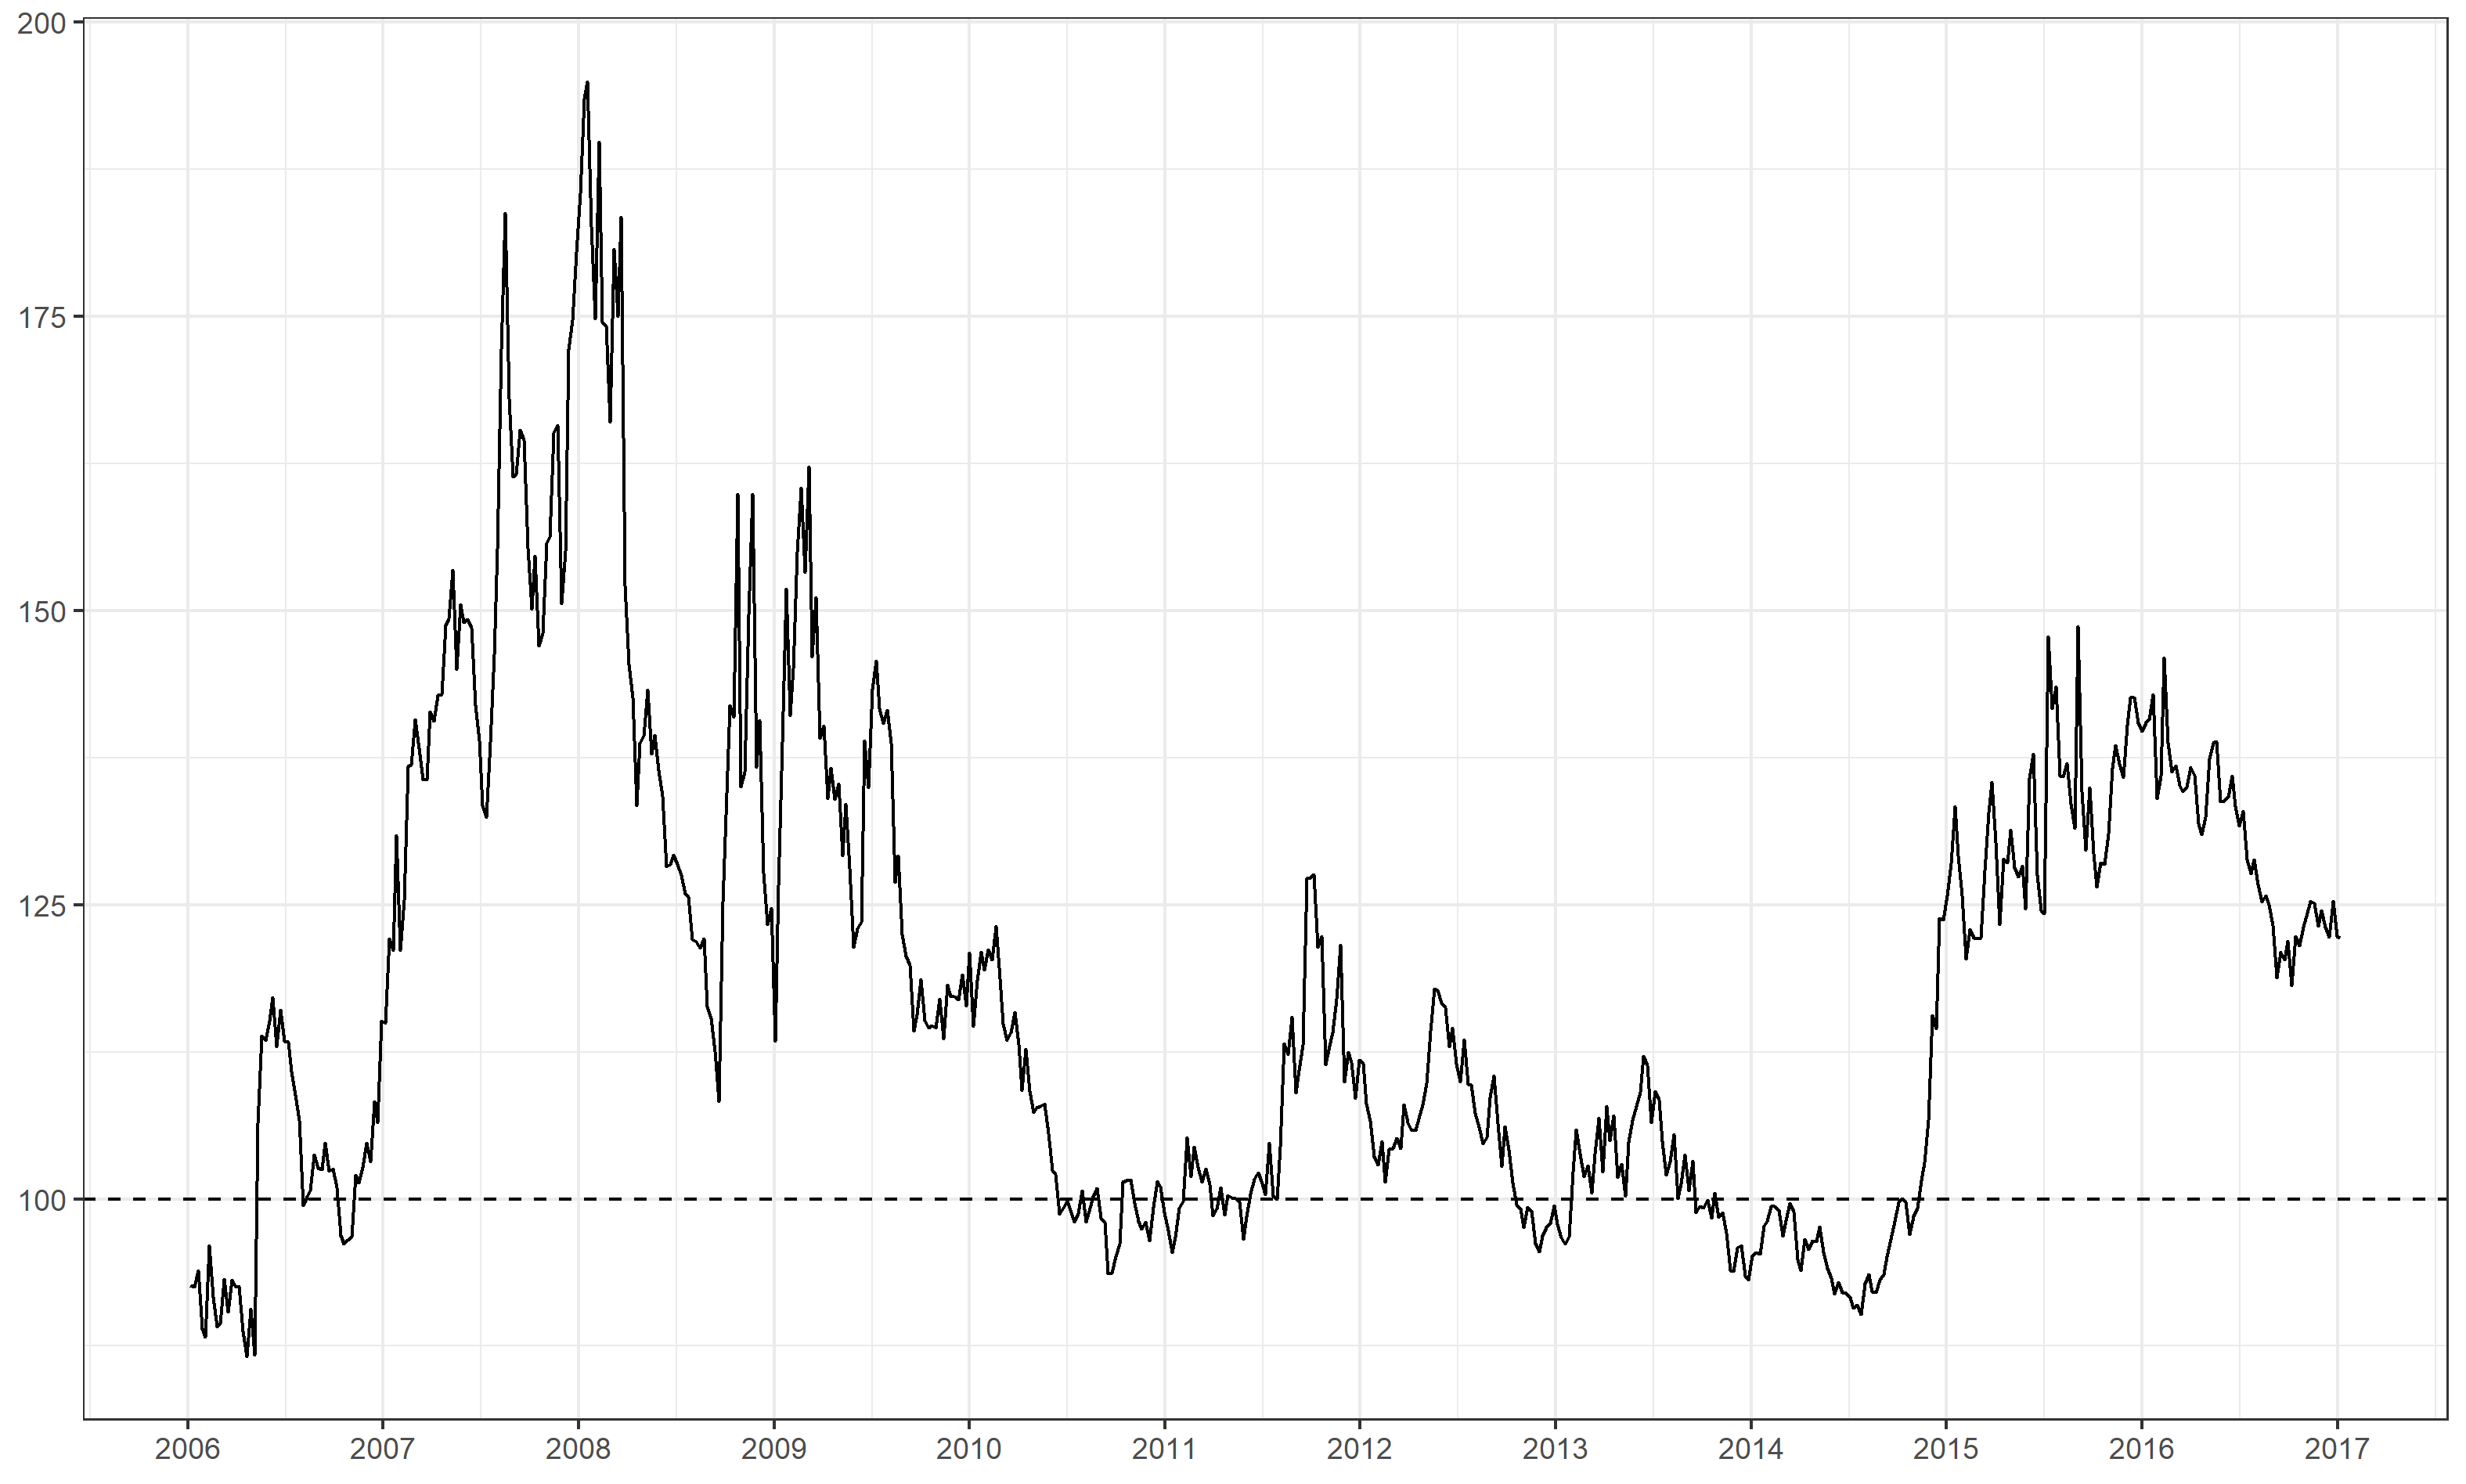
\includegraphics[width = .7\textwidth]{plot-AHind.png}
    % \caption*{\scriptsize \texts{Notes:}}
    \label{fig:AHind}
\end{figure}

%%%%%%%%%%%%%%%%%%%%%%%%%%%%%%%%%%%%%%%%%%%%%%%%%%%%%%%%%%%
\begin{figure}[!htbp]
    \centering  
    
     \caption{\textsc{Date-stamping Periods of Market Exuberance}}
    
    \begin{minipage}{0.48\textwidth}
        \centering
        \caption*{\textsc{AH Premium Index}}
            % \label{fig:autoplot1}
        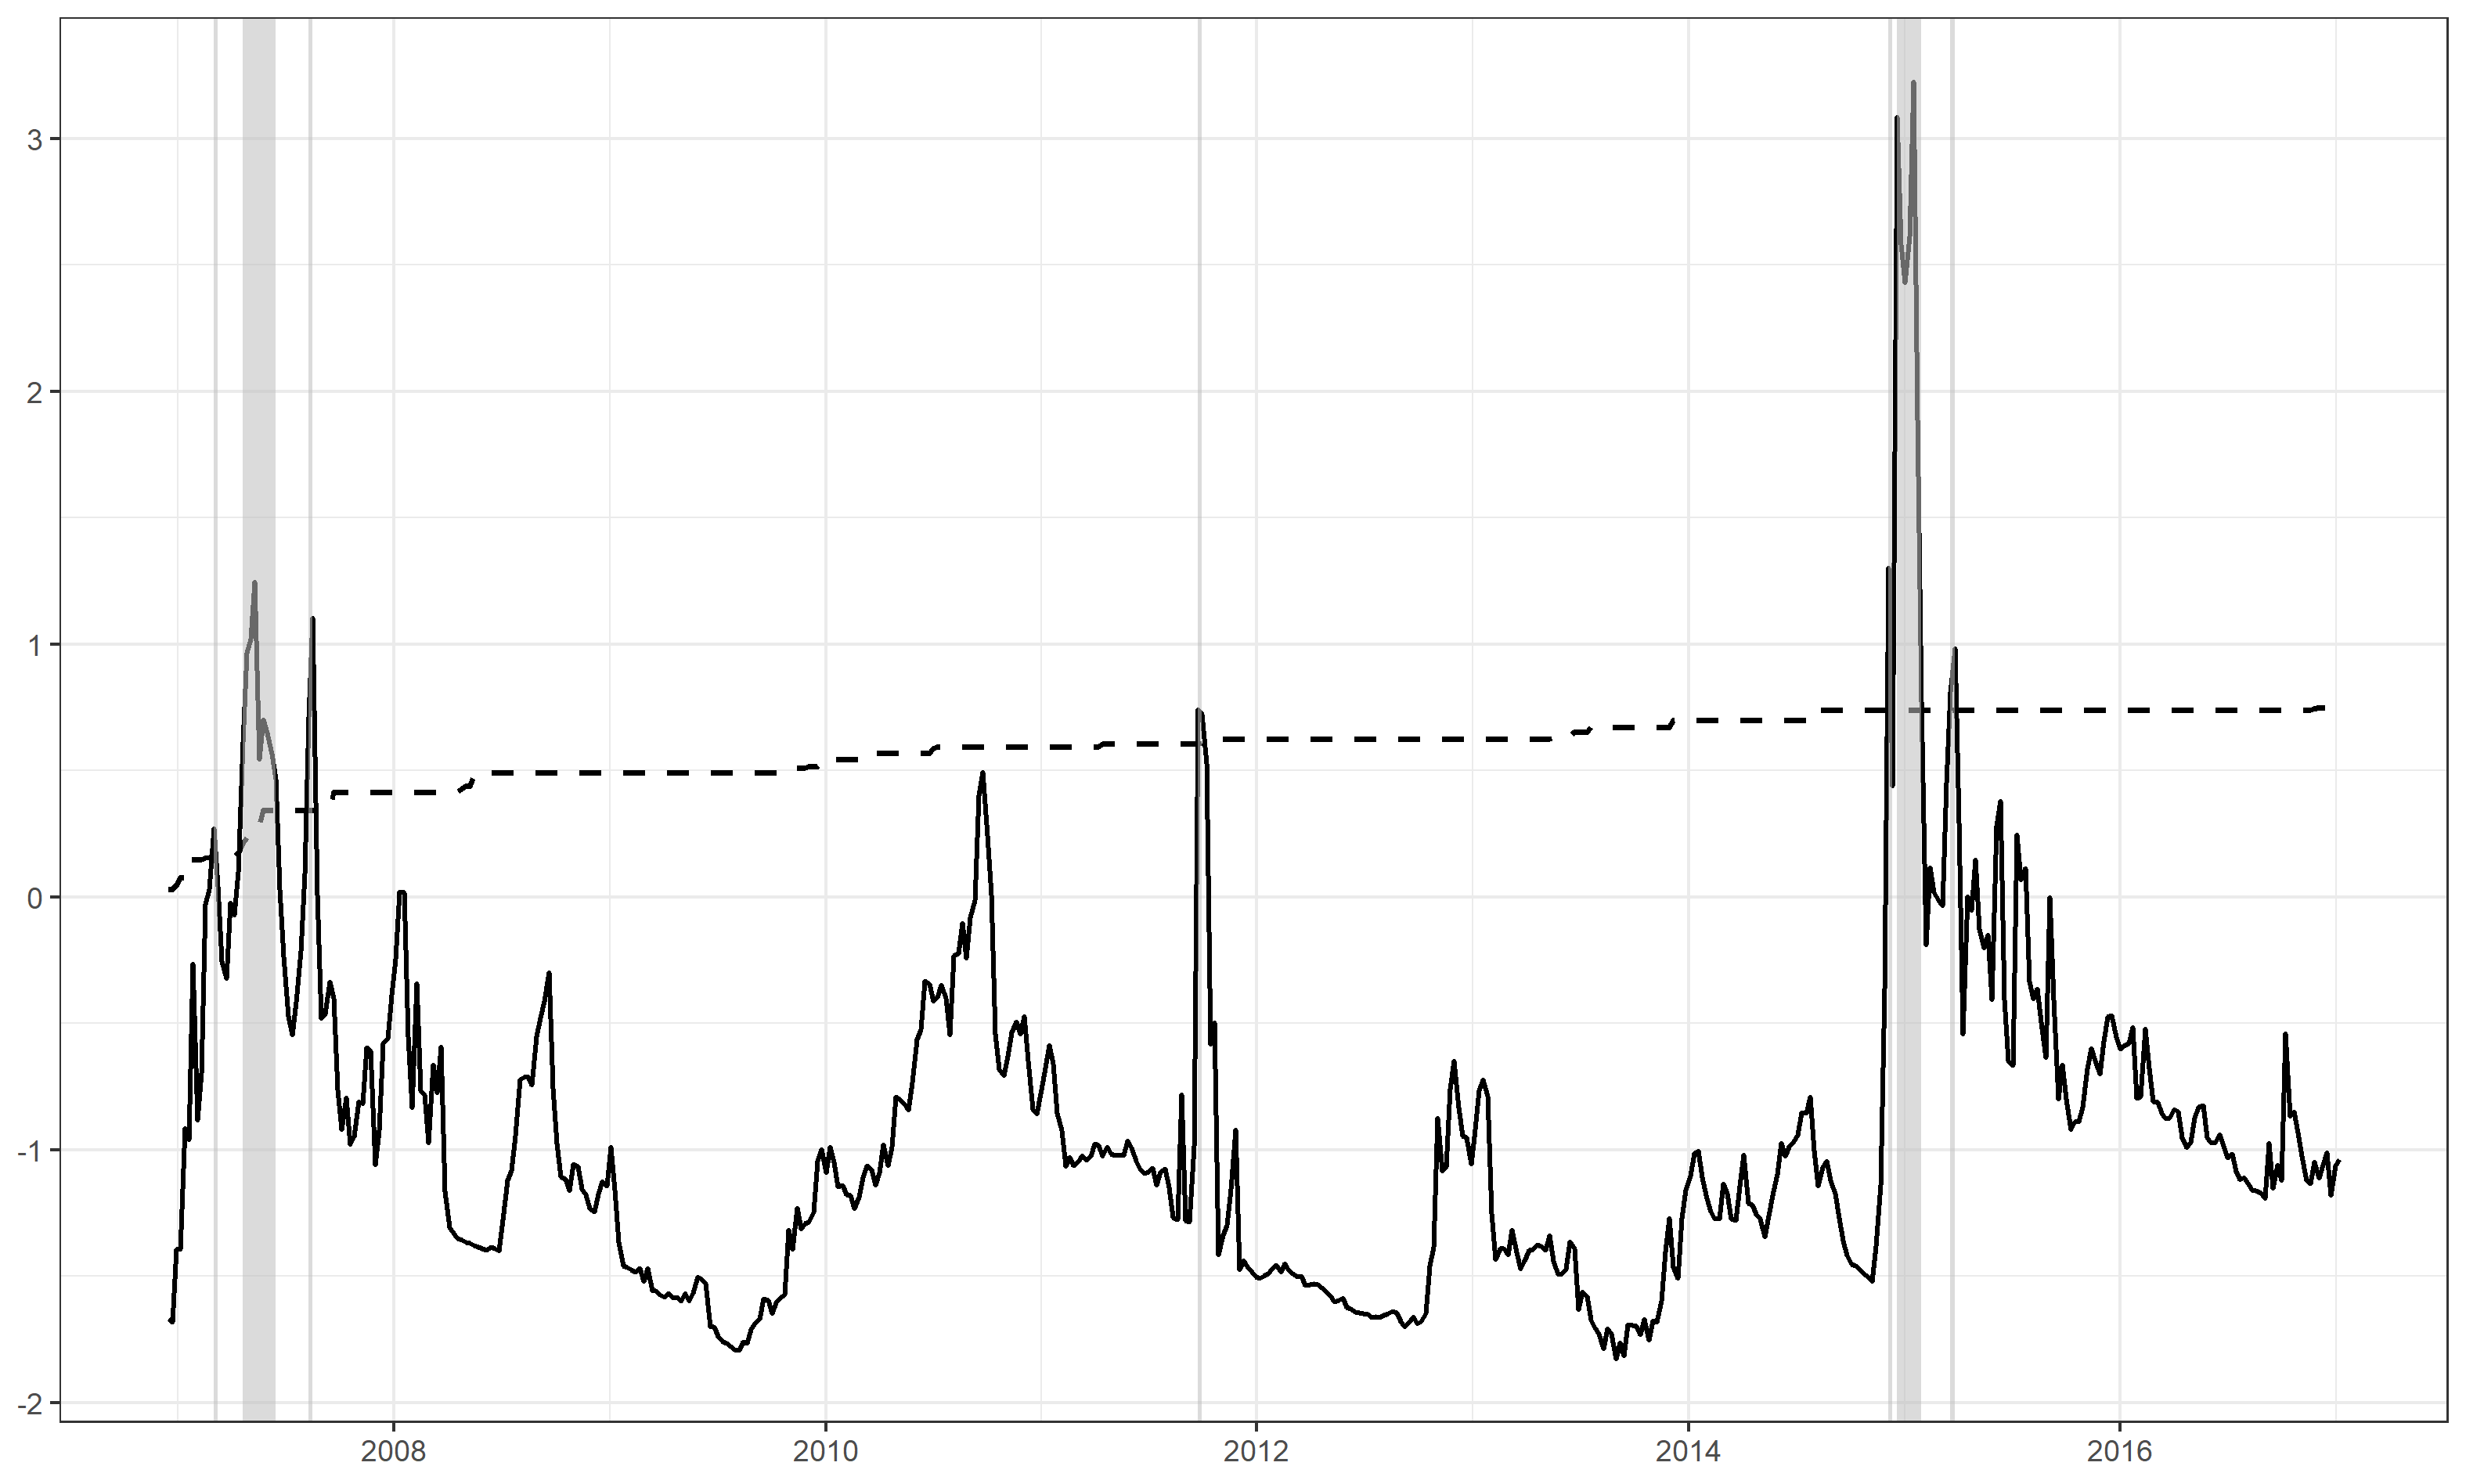
\includegraphics[width=\textwidth]{autoplot-p1.png}
    \end{minipage}\hfill
    \begin{minipage}{0.48\textwidth}
        \centering
        \caption*{\textsc{Panel AH}}
            % \label{fig:autoplot2}
        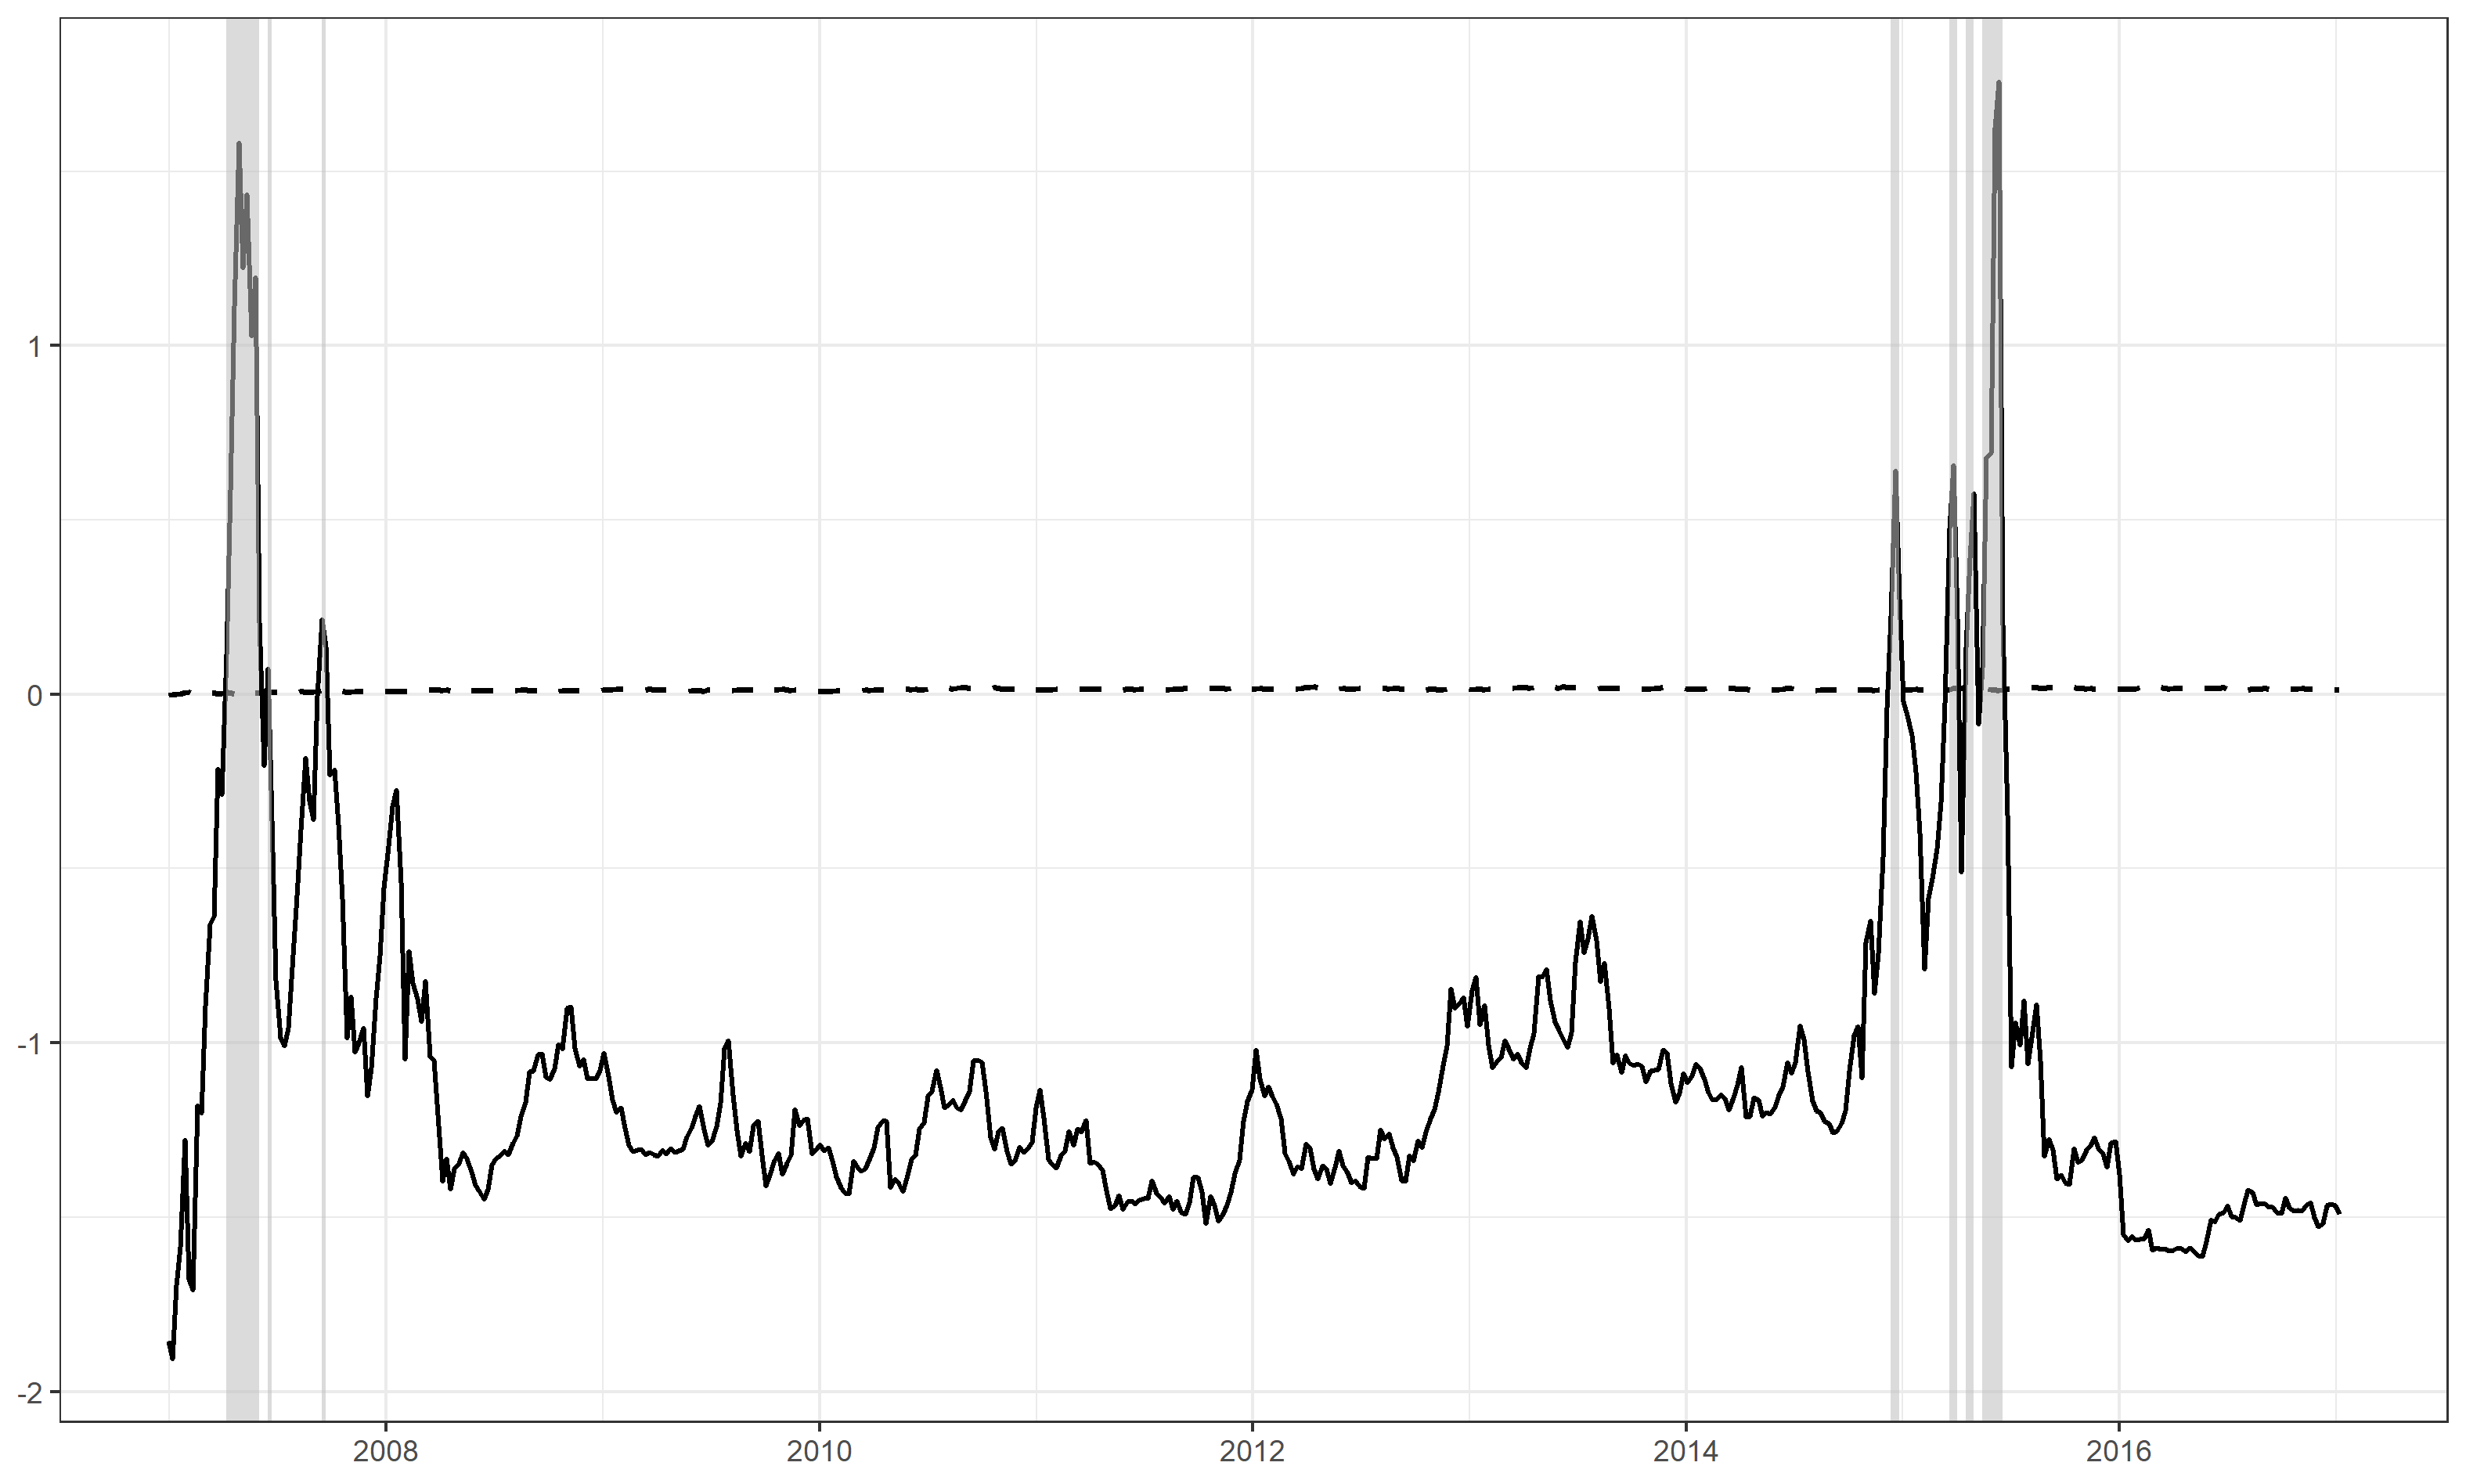
\includegraphics[width=\textwidth]{autoplot-p2.png}
    \end{minipage}\hfill

    
    \caption*{\scriptsize Notes:  The plots display the sequence of BSADF statistics (solid line) together with the corresponding 95 percent critical value sequence (dotted line) for the AH premium index (left) and the panel of 27 cross-listed companies (right). Critical values are obtained using 2000 simulations. The minimum window is 48 weeks. The shaded areas indicate periods of exuberance.}
     
    \label{fig:autoplot}
    
\end{figure}

\begin{figure}[!t]
     \caption{\textsc{Date-stamping Periods of Exuberance in AH Price Differentials}}
     % Date stamping bubble periods in the Hang Seng China AH Premium Pairs
    \centering
    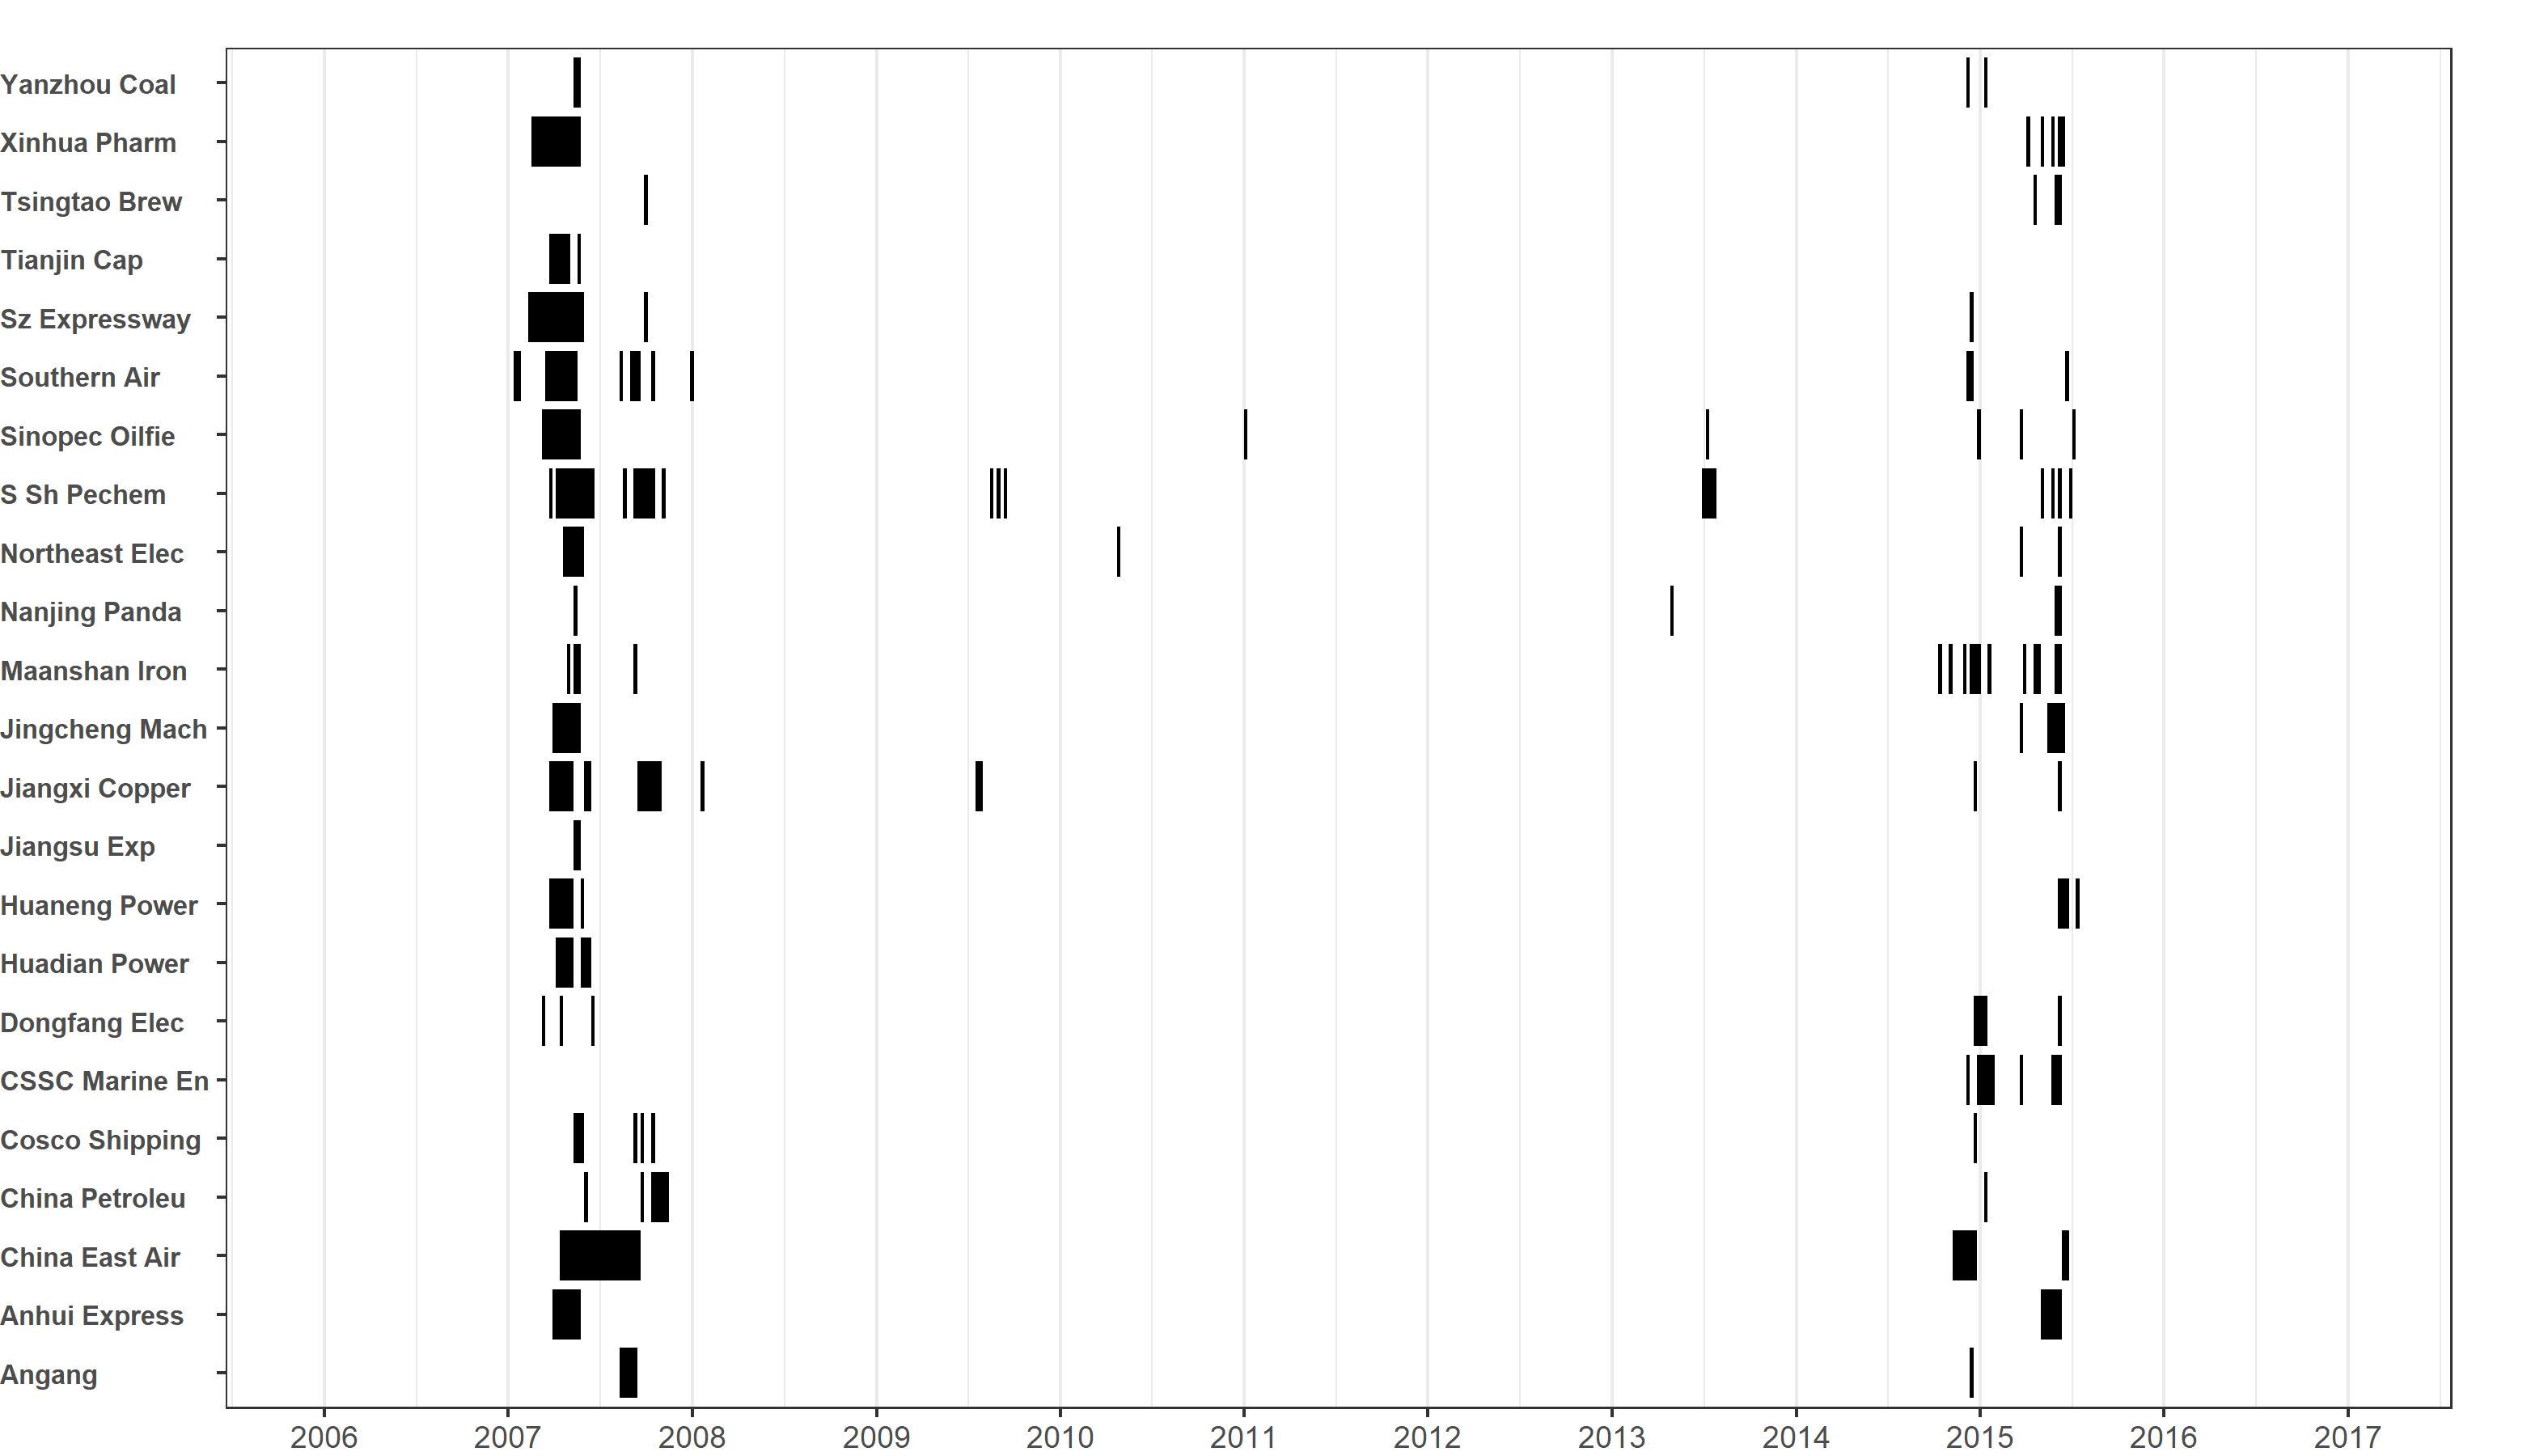
\includegraphics[width = \textwidth]{concordance-AH.png}
    \caption*{\scriptsize Notes: The figure shows the periods of exuberance in A-H share price differentials identified by the BSADF date-stamping strategy. 95 percent critical values are obtained using 2000 simulations. The minimum window size is 48 weeks.}
    \label{fig:datestamp-pairs}
\end{figure}

\begin{figure}[!t]
    \caption{ \textsc{Date-stamping Periods of In-Sample Predictability}}
    \centering
    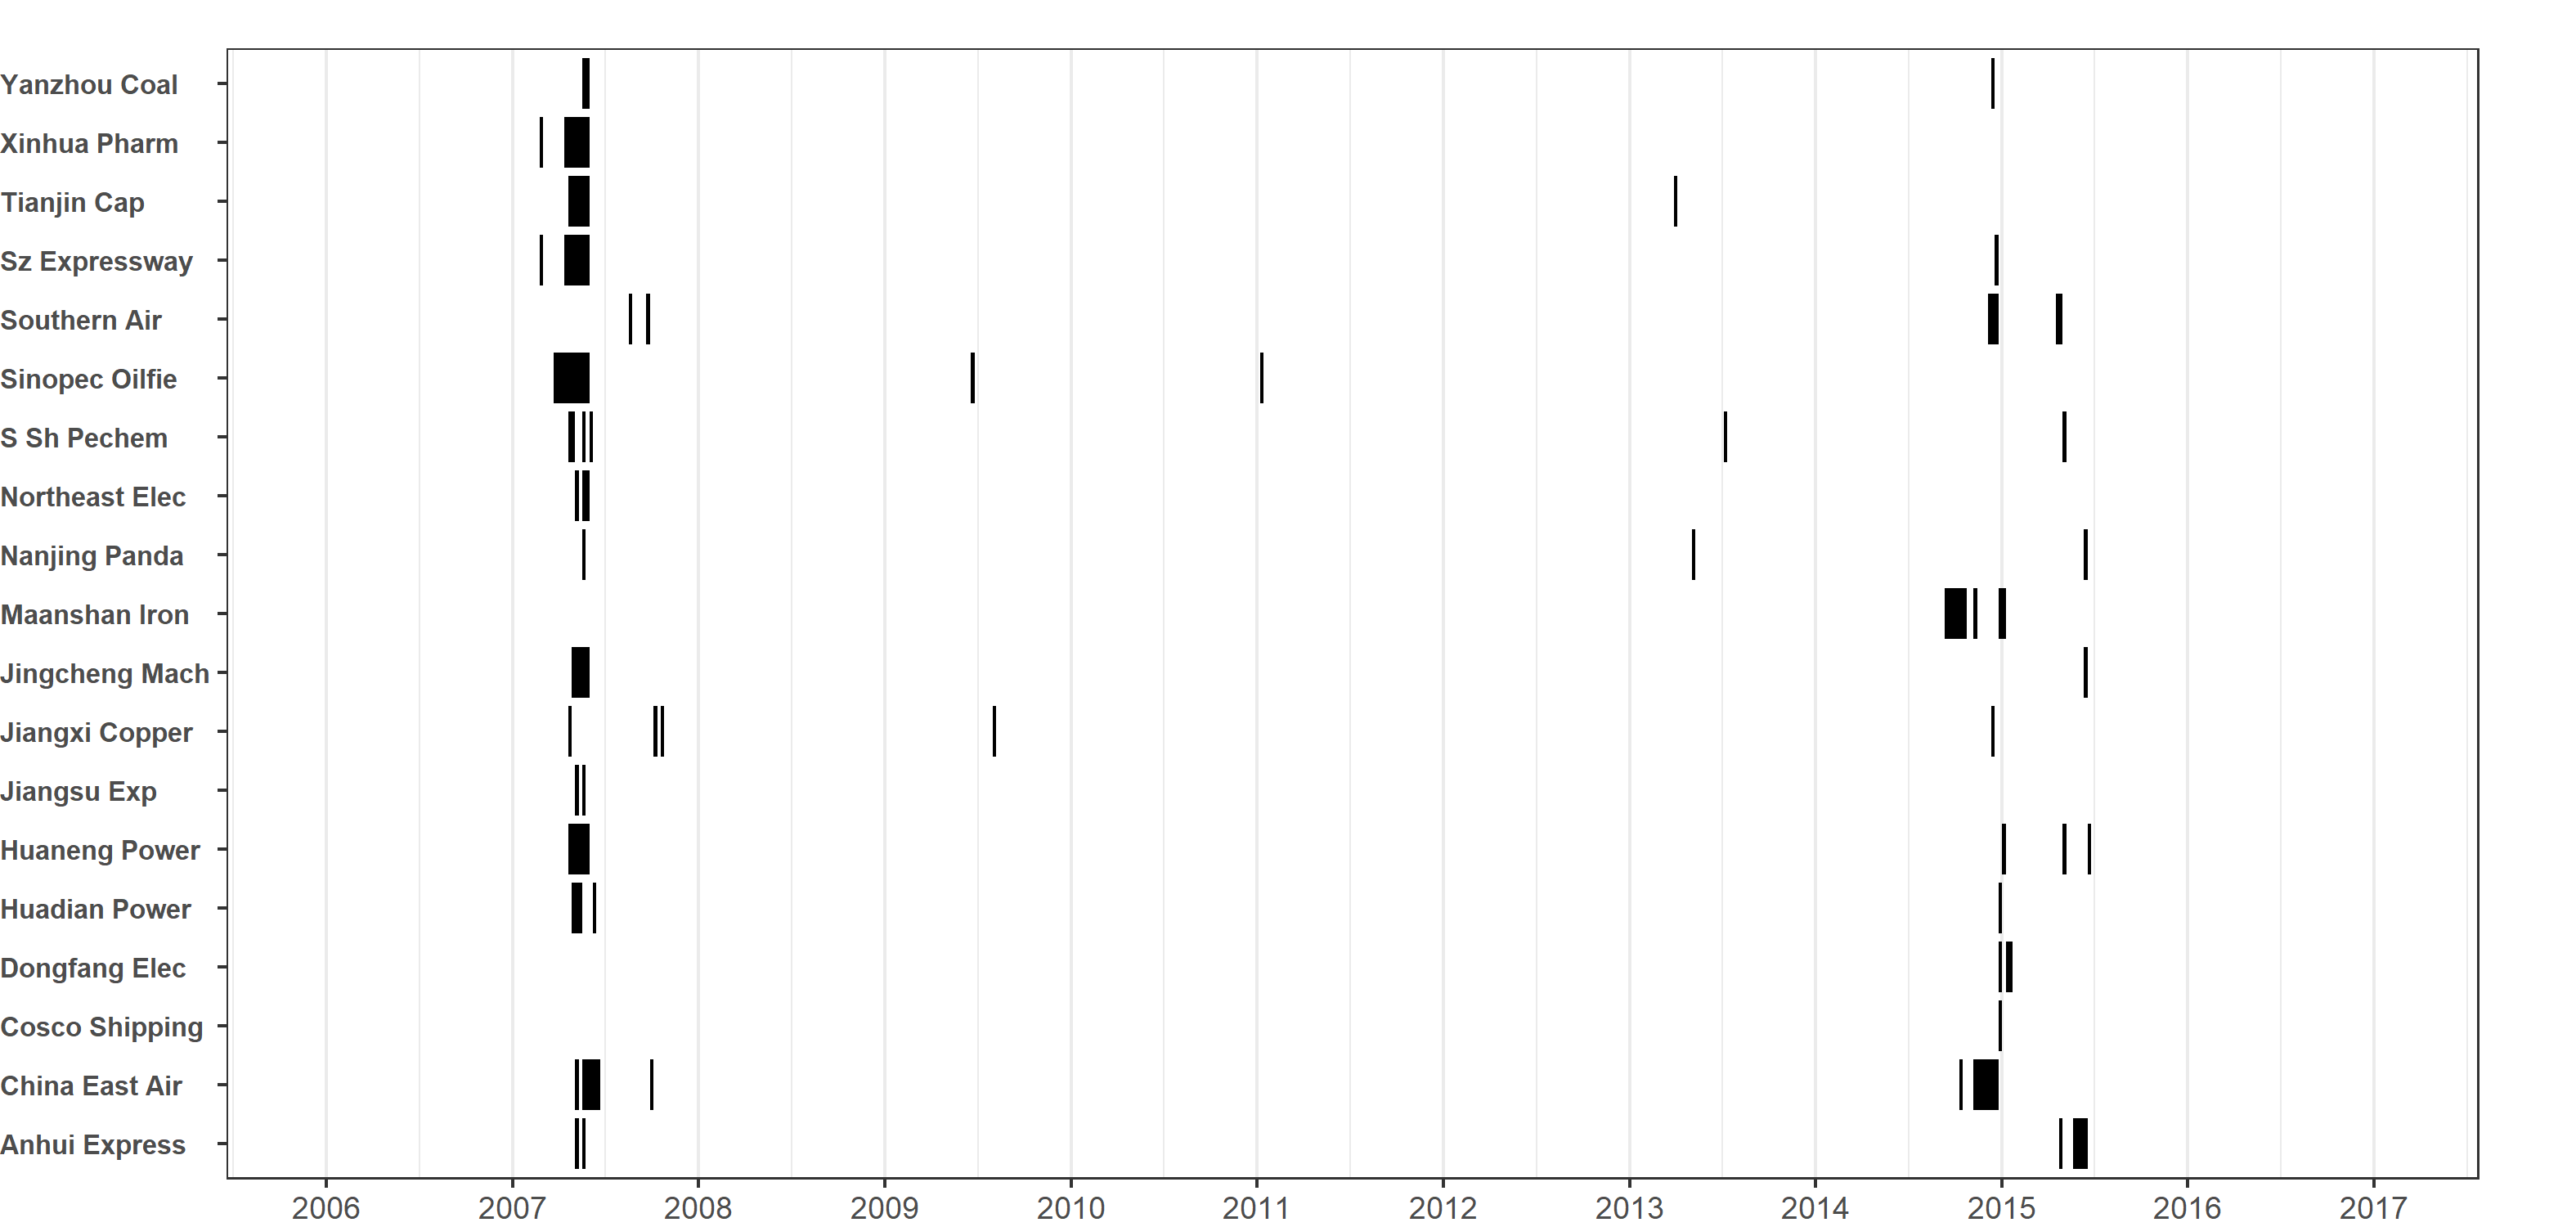
\includegraphics[scale=0.60]{pred-AH.png}
    \caption*{\scriptsize Notes: The figure shows the periods of in-sample predictability of A-share price movements identified by IVX rolling-predictive regressions. The regressor in Equation (\ref{eq:predeq}) is the A-H price differential. The window size is 48 weeks.} 
    \label{fig:pred-AH}
\end{figure}



\begin{figure}[!t]
     \caption{\textsc{Date-stamping Periods of Exuberance in A-ADR Price Differentials}}
     % Date stamping bubble periods in the Hang Seng China AH Premium Pairs
    \centering
    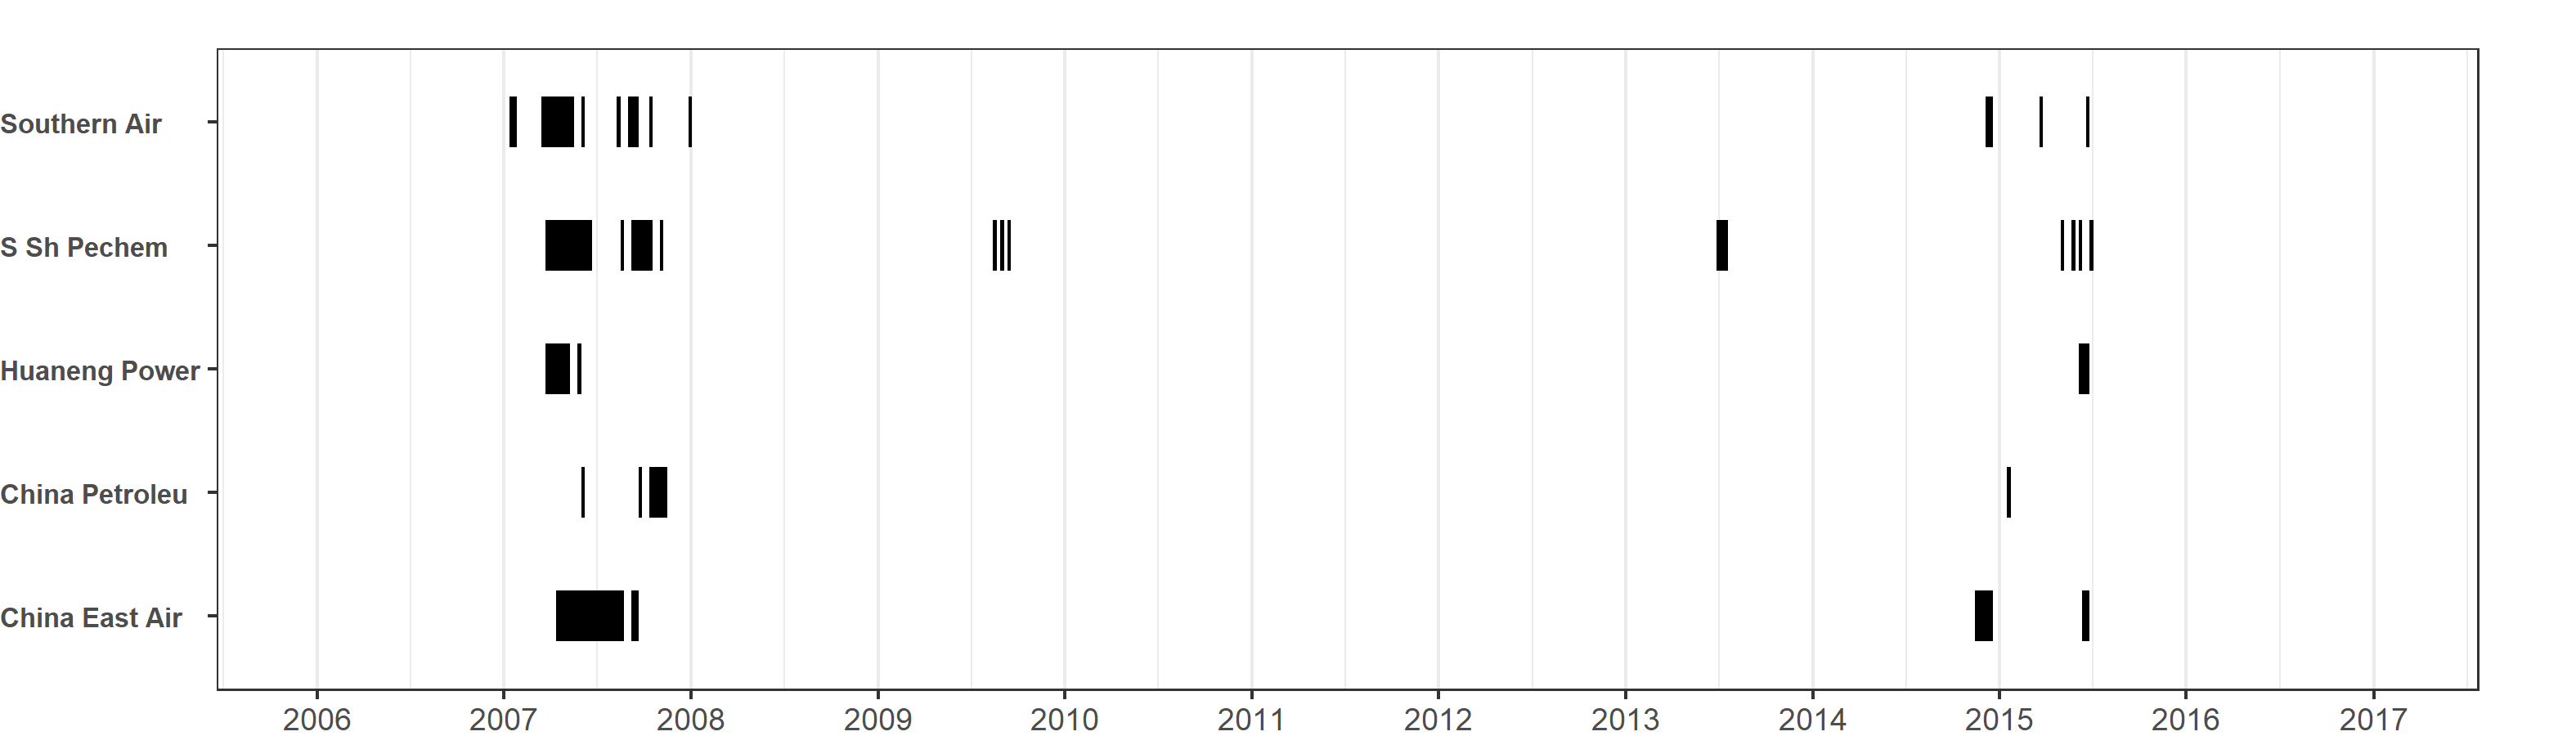
\includegraphics[width = \textwidth,height=4.5cm]{concordance-AADR.png}
    \caption*{\scriptsize Notes: The figure shows the periods of exuberance in A-ADR price differentials identified by the BSADF date-stamping strategy. 95 percent critical values are obtained using 2000 simulations. The minimum window size is 48 weeks.}
    \label{fig:datestamp-ADR}
\end{figure}


\begin{figure}[!t]
    \caption{ \textsc{Date-stamping Periods of In-Sample Predictability}}
    \centering
    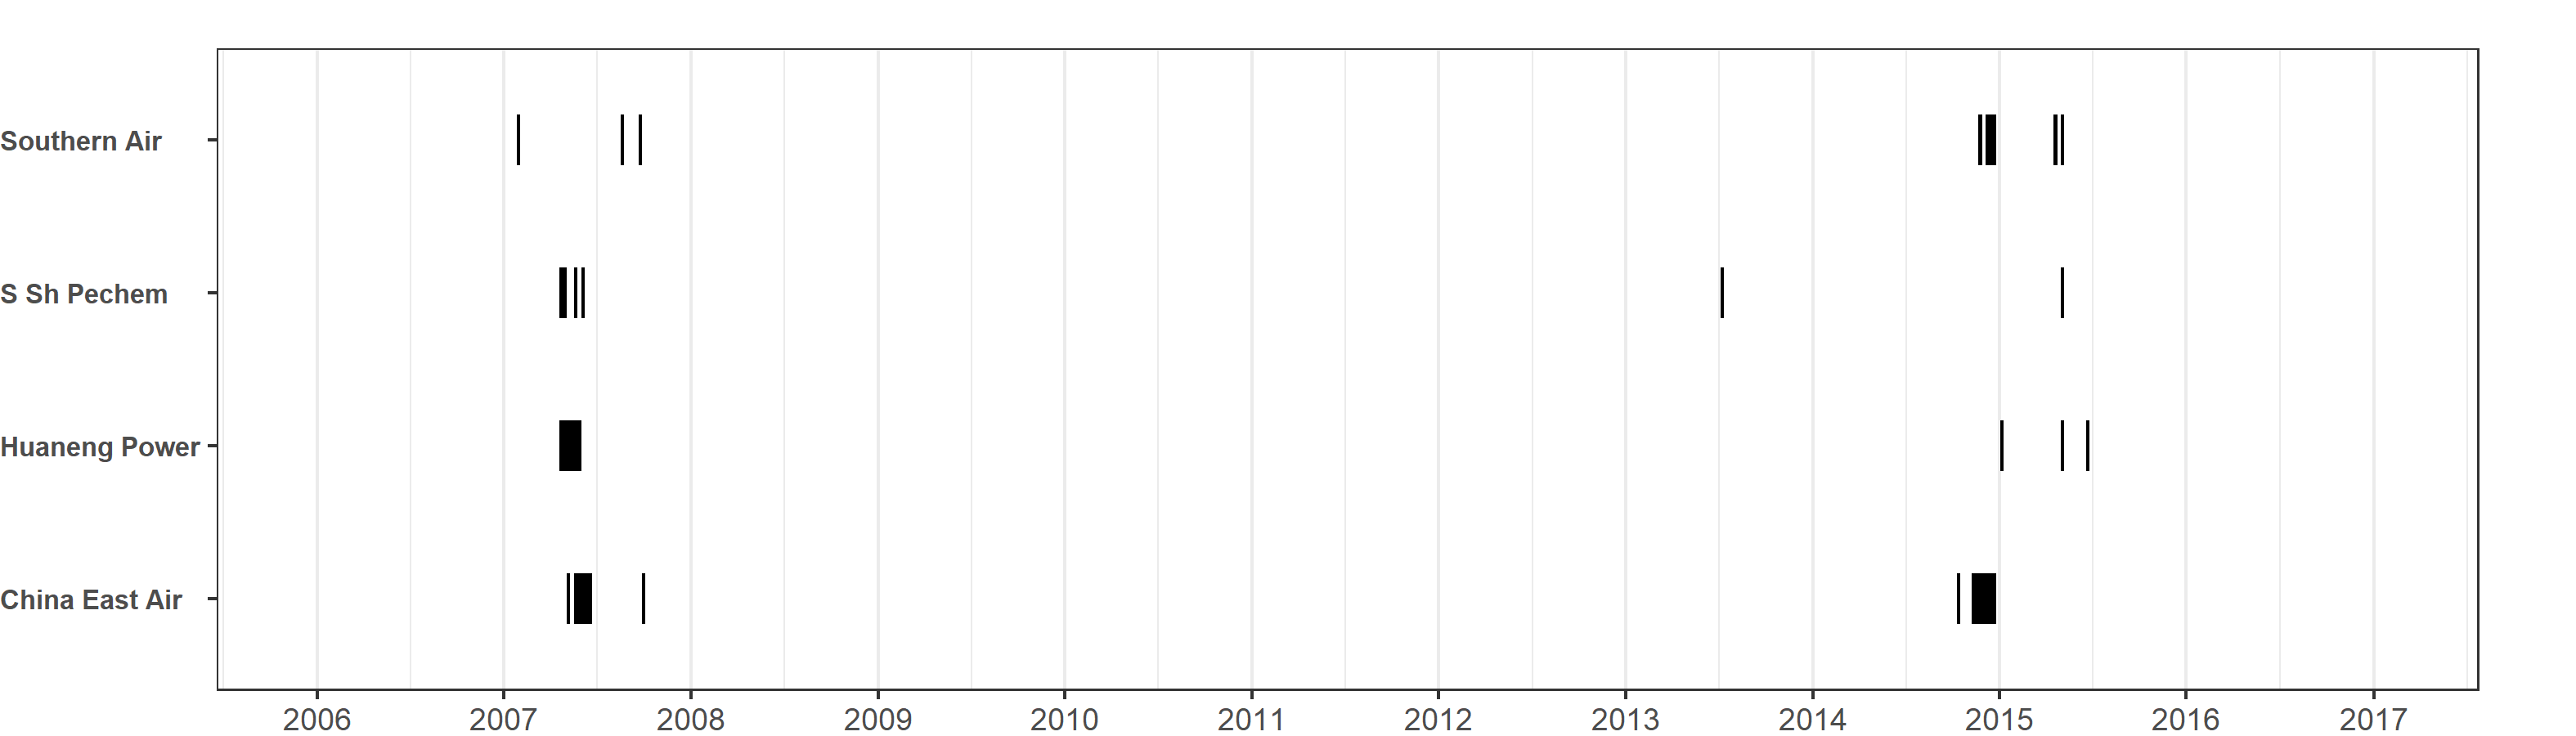
\includegraphics[width=\textwidth,height=4.5cm]{pred-AADR.png}
    \caption*{\scriptsize Notes: The figure shows the periods of in-sample predictability of A-share price movements identified by IVX rolling-predictive regressions. The regressor in Equation (\ref{eq:predeq}) is the A-ADR price differential. The window size is 48 weeks.} 
    \label{fig:pred-ADR}
\end{figure}






\end{document}

